% !TeX root = ./Thesis.tex
\documentclass[10pt,b5paper,twoside,openright]{book}
%Template for project and MSc project reports created by MSc Morten Fyhn Amundsen
\usepackage{config}
\begin{document}

\frontmatter
\pagestyle{plain}
\begingroup


\let\cleardoublepage\clearpage
%Problem description - describing the project tasks, supervisor and co-supervisor - is the first page of the report. For MSc theses, this is generated by the DAIM system. For project reports, you generate this page yourself.
%!TEX root = ../Thesis.tex
\chapter*{\englishproblemname}
\addcontentsline{toc}{chapter}{\englishproblemname}
%
\todo[inline]{Here the problem description  is presented.}
Combustion of municipal  waste comes with the issues of great uncertainty when it comes to the properties of the waste. Noxious gases are released if the combustion is incomplete. As a result, there are strict regulations the maximum concentration of $CO$, acidic gases, like $NO_x$, $HCl$ and $HF$ and heavy metals, like $Cd$ and $Hg$. Since the properties of the waste are inhomogeneous, it becomes difficult to maintain constant steam production

\todo[inline]{Also bad: polychlorinated dibenzodioxins and dibenzofurans}

\todo[inline]{Reffer to "https://www.britannica.com/technology/solid-waste-management" (?)}
\clearpage

%!TEX root = ../Thesis.tex
\chapter*{\englishabstractname}
\addcontentsline{toc}{chapter}{\englishabstractname}
%
\todo[inline]{The abstract is a summary of the contents of the report.}
%

\clearpage


The process of burning MSW\footnote{Manucipial Solid Waste} is a rather complex one, with multiple objectives, non-minimum phase responses long time-constants in combination with very short ones, large disturbances because of varying waste quality. During the last years, stricter regulations have been put in with the regards to the release of hazardous materials. As a result, SINTEF Energy Research has done further research on the subject of modelling and controlling combustion processes. This project attempts to use the additional information that is gained from having a sensor estimating the heating value of the waste, as well as some of the additional information gained from using a more complex model when controlling the plant.
%!TEX root = ../Thesis.tex
\chapter*{\norwegianabstractname}
\addcontentsline{toc}{chapter}{\norwegianabstractname}
%
Sammendraget skal gi en kort oppsummering av innholdet i rapporten.
%
\clearpage

\tableofcontents \clearpage
\listoftables    \clearpage
\listoffigures   \clearpage
%!TEX root = ../Thesis.tex
\chapter*{\englishprefacename}
\addcontentsline{toc}{chapter}{\englishprefacename}

This master's thesis is a part of the requirements for the master degree at the Department for Engineering Cybernetics at the Norwegian University of Science and Technology (NTNU). The thesis was done under the supervision of Associate professor Fredrik Dessen and in collaboration with SINTEF Energy Research under the additional supervision of Dr Elisa Magnelli, and Dr Michael Becidan. 

The thesis is not based on a previous specialization project. However it is based on previous work at SINTEF Energy Research, as well as a report  of a previous summer-student, Herman Øie Kolden. As with all of the reports from the summer-students at SINTEF, the report by \cite{summer_student} was never published. \todo[inline]{Check if the report was ever published}

\noindent
SINTEF provided am in-house simulator developed during the Waste-to-Energy 2030 project, co-funded by industry and public partners and the Research Council of Norway under EnergiX program (WtW, 2030, 280949).

\noindent
The model was expanded to include an implementation of an A/B-controller and a cascaded A/B controller through the work done in \cite{summer_student}. This model was used in chapter \ref{cha:experimental_results}. A Model Predictive Controller had also been developed using one of MATLAB's toolboxes, but due to the relatively long sampling-time, it had no way to keep up with the performance of the A/B-controller. The implementation of the Eigensystem Realisation Algorithm was based on the video-lectures on Youtube by Steve Brunton. All plots were made using MATLAB's built-in functions. The same goes for most complex mathematical operations that have a build-in MATLAB-function, like singular value decomposition, and conversion between continuous and discrete Linear Time-Invariant systems. 


\noindent
I would especially like to thank one of my supervisors, Elisa, for taking time out of her day, helping me with the mysterious problems that resulted from the simulator. Also, I'd like to thank Fredrik, as well, for answering most of my control-related questions and for advising me to take more time, so that I could deliver a more functioning product. Finally, I'd like to thank my family for giving me the time, space and support needed for completing this project. 

\hfill {\it Jørn Bøni Hofstad}\\[-6mm]

\hfill {\it Trondheim, August 2020}
%

\clearpage

%List of Acronyms and List of symbols can be useful to include if you have many.
\endgroup

\mainmatter
\pagestyle{headings}
%!TEX root = ../Thesis.tex
\chapter{Introduction}\label{cha:introduction}
%


\todo[inline]{
This introductory chapter will briefly provide context for the material/results presented in this report and give motivation and a description of the problem to be solved. A literature review summarises existing relevant knowledge and establishes the foundation of the later control system. The scope of the work is then defined through a list of assumptions. Finally, the contributions of the thesis are defined and elaborated.}



\section{Motivation}\label{sec:motivation}

Combustion of Municipal Solid Waste(MSW) is a process that has gained increased attention in the last years. This is both as a result of a steady increase in produced waste, as well as stricter regulations, which means that the plants have to follow stricter standards with regards to both gas emission and management of the solid ash left behind after the combustion. One way to ensure all conditions are met is to find some operating point that is know for causing the system to behave in the desired manner, and then using a controller to make sure the system stays near that state, regardless of any disturbances that may affect the process. A solution using cascaded PID-controllers has already been made by SINTEF. But that model will not be able to take full advantage of how to combine different inputs in such a way disturbances are suppressed, while not affecting other outputs too much. 

\subsection{Literature review}
There has already been quite a bit on work on the subject of waste incineration, like in \cite{waste_prof}. Furthermore, there has been some interest in using additional sensors to the ones that are normally used when controlling such a plant. In \cite{summer_student}, an estimate of the heating value was used to give a controller that could handle changes in waste-quality more effectively. \cite{waste_prof} tested several different implementations for how to control waste-combustion plants. Waste-incineration suffers from the typical problem that when one tries to increase one of the measured variables by increasing one of the inputs, there will usually be a rather large overshoot, as well as some states decreasing before they start to increase again. This is what is known as a non-minimum phase system and they are usually more difficult to control. Furthermore, changing one input usually affects all outputs. This makes it so that there are other controllers than PID-controllers that may be able to give better results. This thesis will attempt to improve on the solution in \cite{summer_student} by estimating a system with the method given in \cite{ERA_source}, and then combining the acquired model with standard linear dynamical systems theory, like what is found in \cite{cont_LQR_lecture} to make a better controller. Finally, the estimated model may also be used for gaining a feeling for how sensitive the rest of the system is to disturbances, measurement  and modelling errors. The method will be repeated on a selection of different model-based linear controllers with slightly different architecture  to find the one that has the best performance while also having some indicator of its robustness. 
\todo[inline]{Make sure I do this...}

\subsection{Assumptions}
Since the main implementation is based on a linear model, the biggest assumption about the plant is that it behaves sufficiently similar to a linear time-invariant system. Furthermore, it is assumed that any time-delay in the control-loop remains within certain borders. Additionally, it is assumed that all modelling errors are on the form of pure time-delays or in the form of incorrect scaling for the input-matrix $B$, and that these errors vary so slowly that they can be seen as piece-wise constant when stabilising the plant and that these periods are so long that the controller gets the time to stabilise the plant. The implementation that was used also assumes that the process disturbances have a much larger effect on measured signals than the measurement-noise as long as a low-pass filter with a cutoff-frequency of $1 \left[\frac{rad}{s}\right]$ is used. However, this assumption can be changed later by using a new filter and re-tuning the weights in the controller and the state estimator. 
\subsection{Contributions}
The contributions from this project mainly come in the form of implementations of the different controllers, as well as an implementation of the Eigensystem Realisation Algorithm. All steps needed for the algorithm to work can be found in \cite{ERA_source}. Two different estimated systems were implemented. One that only considers how the controlled disturbances affect the outputs, and one that also uses the measured disturbances from the simulation to give an optimistic estimate of the increase in performance if they could be measured. It can also be used for getting a better estimate of how the process-disturbances affect the output, which can be used when designing the estimator. 

\noindent
Making a Linear Quadratic Estimator that is decoupled form the rest of the controller also allows for properly utilising the sensor measurements for state-estimation, since a Model Predictive Controller needs more computation time than a Kalman filter. 
\noindent
Finally, some different controller architectures were explored, which had the purpose of making the controller follow the desired steady-state, since some combinations of inputs can only be allowed to handle transient inputs, and should not be used to make the controller reach its steady-state. Finally, some robustness analysis was also done on the linear, estimated system to give some kind of guess to how robust the controller might be. 

\subsection{Outline}
The thesis is divided into $N$ chapters. 

\begin{itemize}
  \item \ref{cha:process_overview}: Process overview 
  \item \ref{cha:characteristics_of_process}: Features of the process 
  \item \ref{sec:ERA}: Parameter estimation
  \item \ref{cha:controllers}: Controllers
  \item \ref{cha:experimental_results}: Experimental result
  \item \ref{cha:conclusions}: Conclusion and future work
\end{itemize}




Chapter \ref{cha:process_overview} will explain what happens in the process, without going in-depth about what mathematical model is required to simulate the given system. This is mostly due to the complexity of a combustion process, which results in a proper explanation of how the process works being outside the scope of this thesis. 


\noindent
Chapter \ref{cha:characteristics_of_process} will cover the qualitative properties of the system's step responses when the system is excited around the operating point. This may give some information as to what issues will be the most pressing when trying to control the plant. 


\noindent
The different controller architectures will be discussed in chapter \ref{cha:controllers}, namely two PID-controller architectures, as well a few methods for optimal control. Namely, the Model Predictive Controller and the Linear Quadratic Regulator. Different architectures can be tested, depending on if there is supposed to be some kind of cost on the system for excessively increasing the primary air while reducing the secondary air. 


\noindent
Chapter \ref{cha:experimental_results} describes the process of tuning the controllers, as well as how the resulting closed-loop system respond to disturbances and noise. Because of the system being somewhat inaccurate when it comes to representing how the system will most likely act in reality. 
\todo[inline]{Add a part where all disturbances can be measured (?)}
\noindent
Finally, Chapter \ref{cha:conclusions} covers suggestion for future work that could expand and improve the results of the current project. 

% What is the motivation for considering the problems/question that you approach in your work? Why is this an interesting problem? The motivation should instead describe why it is interesting from a societal point of view, and/or from a scientific point of view.}
% \todo[inline]{Remember to cite what has been done earlier on the topic, to put your work in the correct context: In \cite{Adaptiv_boken} a control law is defined which..., while \cite{Adaptiv_boken} considers the particular case of... However, in these works... and in this work, we will extend this by... / we will instead... In "Reference to your own pre-project" a literature review was performed, showing that there is a need for ... }
% \todo[inline]{Moreover, a preliminary controller was developed... but has the drawback that... In this thesis, we will instead ... / we will further develop this control law by utilising the control method XX... 
% }
% Figures are referred to as follows: In Fig.~\ref{fig:curve} you see an interesting curve. There is also a table in this sample report: Table~\ref{tab:a-table}.

% \subsection{A Subsection}\label{ssec:a-subsection}


% \subsubsection{A Subsubsection}\label{sssec:a-subsubsection}

% \lipsum[2]

% \begin{figure}[htbp]
%   \centering
%   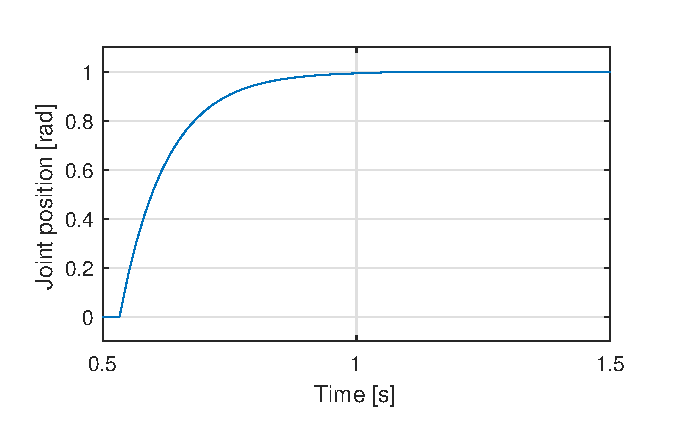
\includegraphics[width=.7\textwidth]{img/time-constant}
%   \caption{The time evolution of the joint angle $q$}
%   \label{fig:curve}
% \end{figure}

% \begin{table}[htbp]
%   \centering
%   \caption{A table}
%   \begin{tabular}{cc}
%     \toprule
%     Something & Something else \\
%     \midrule
%     A & a \\
%     B & b \\
%     \bottomrule
%   \end{tabular}
%   \label{tab:a-table}
% \end{table}

% \section{Literature review}\label{sec:review}

% \section{Assumptions}\label{sec:assumptions}
% Include this section if it is necessary to state some assumptions that you have made to restrict the scope of the thesis.

% \section{Contributions}\label{sec:contributions}
% Here you describe the main contributions of your work: What are the new results - the achievements - of your work on the master project. For instance:
% The main contributions of the work presented in this thesis are as follows:
% \begin{itemize}
% 	\item The development of a control law for ...
% 	\item The development of a simulator for...
% 	\item A simulation study evaluating the performance of the proposed control method.
% 	\item Experimental validation of the theoretical results, using the autonomous ground vehicle...
% \end{itemize} 
% Elaborate on each item/contribution - this is an opportunity for you to convey to the reader (and the examiner) all that you have done during your master´s project work.

% \section{Outline}\label{sec:outline}
% The report is organized as follows. In Chapter~\ref{cha:characteristics_of_process} a mathematical model is developed to describe the system... In Chapter

          

\chapter{Process overview}
 \label{cha:process_overview}
\todo[inline]{This is where the results are supposed to go, so there should be an introduction to them}
A detailed description of the dynamic model used in the present work can be found in \cite{Elisa_source}.
As a result, there will only a quick summary of the process will be given in this thesis. 

\section{Process overview}

\begin{figure}[htbp]
    \centering
    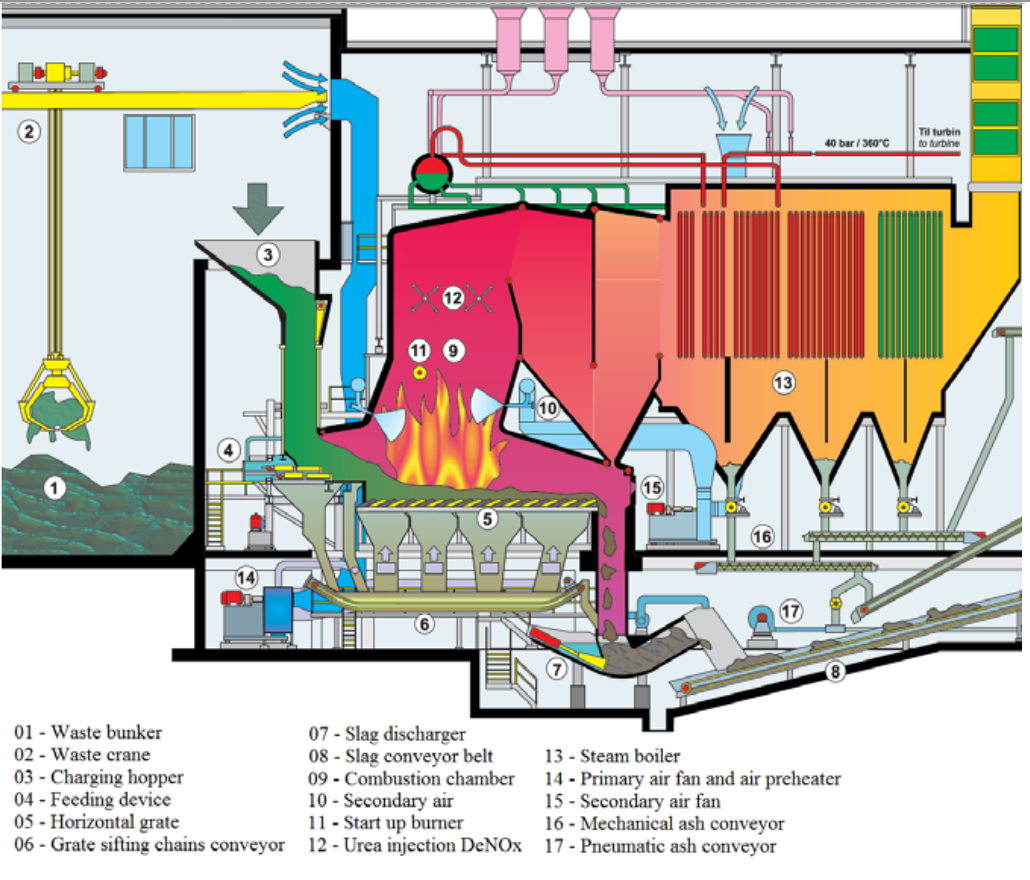
\includegraphics[width=\textwidth]{img/plant_overview.png}
    \caption{Overview of the plant}
    \label{fig:plant_overview}
  \end{figure}
  

As seen in Figure \ref{fig:plant_overview}, the waste is normally delivered to the waste-bunker (1). There, a set of cranes are used to mix it, to make it more homogeneous, decreasing how much the waste-composition varies, and therefore the disturbances. Some of it is then fed into the charging hopper (3) by the same cranes. A ram (4) pushes the waste onto the waste-grates (5). While on the grate, the primary air-flow (17) dries the waste and provides oxygen for the primary combustion. The conversion process taking place on the grates can be seen as divided into three sections. The waste is dried in the first section. On the second section of the grate, the primary combustion happens, where most of the heat is produced. The third part of the grate, any post-combustion happens to ensure that the amount of combustible material in the ash is below a certain threshold\footnote{In addition to the environmental damage that may come from exceeding these limits for too long, the limits are also enforced by law}. The non-combustible ash is then removed(17) from the system to be cleaned and disposed of. The combustion also results in the production of various gasses, which together with the air that did not react make up the  flue-gas. Somewhere above the second part of the grate, a secondary airflow is also applied to the volatile gases resulting from the primary combustion. This is where secondary combustion occurs, producing more heat through the further conversion of the gases produced by conversion on the grate (e.g. $CO$, $H_2$ and $CH_4$). The primary and secondary airflow(10) provide oxygen to the fire so that the combustion is complete. The two air-flows are added at two different points to allow for better mixing between flue gases and oxygen. Proper mixing is a requirement for having complete combustion and for reducing the formation of $NO_x$ and other harmful gases. The heat-exchange between the burning waste and the flue gas happens through contact, the mass-transfer of gases produced during combustion and by radiation. The flue gas in the combustion chamber(9) has a temperature of roughly $850^O C$. By law, the flue gas need to stay above $850^O C$ for at least 2 seconds. This is to ensure that no dangerous gases are produced. The flue gas travels through multiple bends, called passes. The passes make up the first section of the boiler (i.e. evaporator). The walls in the passes are made up of pipes where saturated water flows. When the gas flows past the pipes, it gives off heat to the walls, turning the saturated water  into saturated steam.  The second part of the boiler(13) (i.e. superheater) , is where the gas is used to heat a flow of saturated steam that is extracted from the boiler drum.  The final heat exchange section is called the economizer. Here, the cold water that is feed into the boiler drum is pre-heated to better take advantage of all the heat in the flue gas. Finally, the flue gas exits out of the system that is to be controlled in this thesis and into the part of the plant where it is cleaned before being released into the atmosphere. The composition of the flue gas that is released will depend on the amount of oxygen, how well oxygen and flue gas was mixed during combustion, the temperature in the combustion chamber, as well as the composition of the waste that is being burned. 

% \chapter{Theory}

% There are several ways to control a process, depending on its properties. Some of them require a model of the process to be known, others require the system to behave close to linearly within the region of operation. Depending on the method chosen, the sensitivity to noise, disturbances and modelling errors may also vary quite a lot. The waste incineration plant is a process containing unmeasured disturbances due to the varying composition of the waste, as well as the complex dynamics involved in combustion and the movement of fluids. All of these factors may prove to be problematic. The following chapter will cover a set of different methods potentially modelling a process, as well as how to control it. 

\chapter{Features of the combustion process}
\label{cha:characteristics_of_process}
% \cite{waste_prof} provides a model for describing the combustion process in a plant. However, according to \cite{Elisa_source}, the model suffers from being imprecise. Especially in regards to the lag of the model, as it was described as being too fast. As a result, the mathematical model can not be used directly. Still, by looking at how the system responds to certain step-inputs, some properties of the system can still be inferred. 


\section{Input step-responses}
\begin{figure}[!ht]
    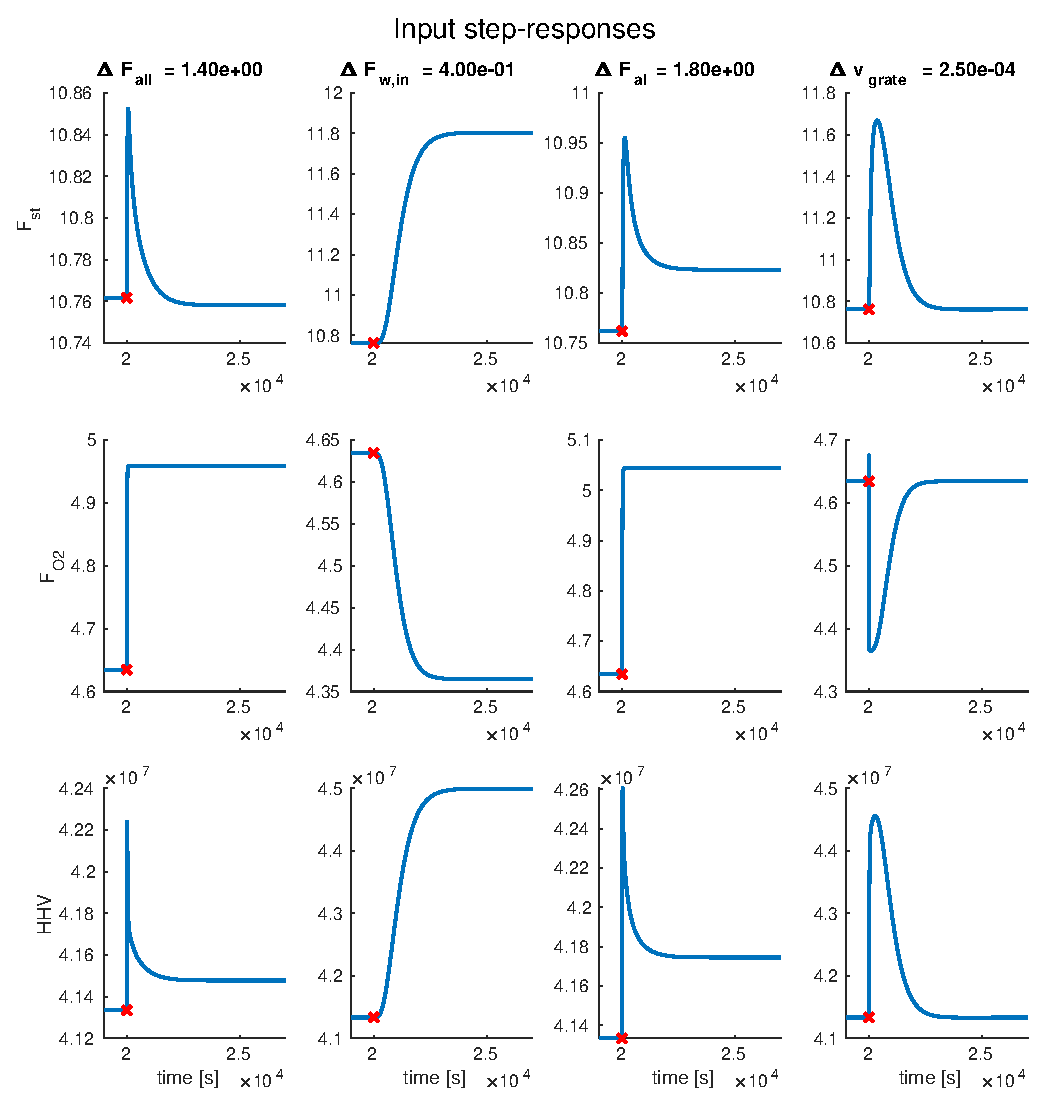
\includegraphics[width=\textwidth]{img/Simple_analysis_plots/Unscaled_input_step_responses.eps}
    \caption{Step-response form the Maniplulable inputs}
    \label{fig:Input_step_response}
\end{figure}

Before doing some actual system identification, it might be useful to do some experiments to get an overview of how the system behaves, as it might give some intuition as to how to control the plant. Figure \ref{fig:unscaled_Input_step_response} shows the result of an experiment  where the first 19000 seconds were used to allow the plant to reach a stationary point, while a constant input-value was held, without any disturbances. At 20000 seconds, one of the input-variables is increased. The point at which the step occurs is shown as a red cross on the graph. Both the inputs and the outputs operate at completely different operating points, and with at completely different orders of magnitude. To better illustrate what is going on, figure \ref{fig:Input_step_response} shows a scaled version of the step-response, where the operating point has been subtracted and the output have been scaled to correspond to what "would have been" if the step-amplitudes had been unity instead. 

\todo[inline]{Different formulation than Manipulable (?)}
\begin{figure}[!ht]
    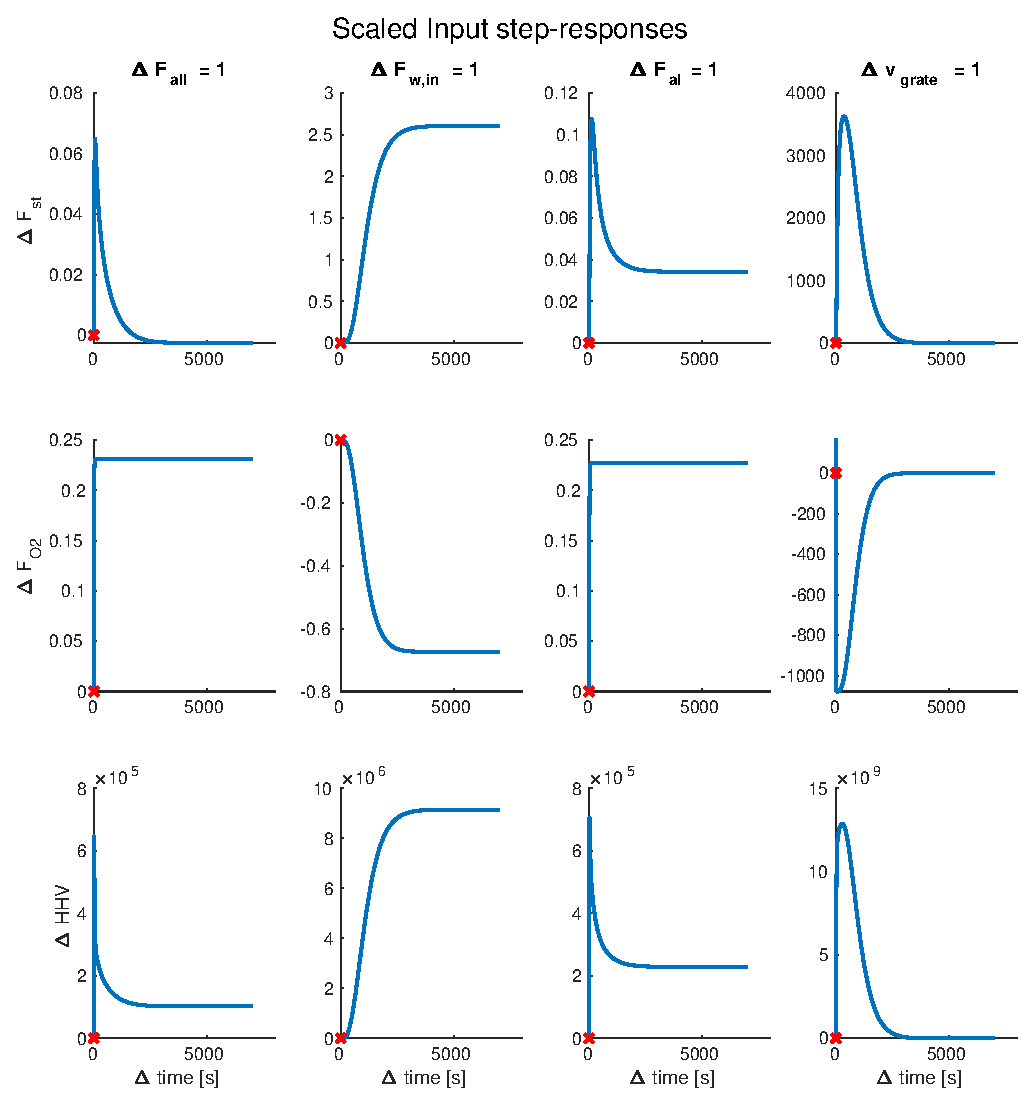
\includegraphics[width=\textwidth]{img/Simple_analysis_plots/Scaled_input_step_responses.eps}
    \caption{Change in outputs, given step-changes in the inputs. Adjusted for the operating point, and scaled for the step-amplitude}
    \label{fig:unscaled_Input_step_response}
\end{figure}

\noindent
As can be seen from figure \ref{fig:Input_step_response}, the speed at which the plant reacts with is very different, depending on the input and the output. The steam-production normally reacts rather slowly to any changes in the amount of waste fed into the plant. This is usually in the realm of thousands of seconds. On the other hand, changing the input of primary or secondary air works almost instantaneously on the mass-flow of air, while also having a fast effect on the steam-production. 

\noindent
The primary air is already pre-heated. Additionally, an increased flow of oxygen flowing through the waste also helps to make more oxygen available for the primary combustion process, which speeds up the process. \cite{Elisa_source} explains that increasing oxygen concentration increases the reaction rate. The effect rapidly decreases again, as the available waste/gases are "used up". 
\noindent

\todo[inline]{@@@ Refer to the article for why the secondary air helps}
\cite{summer_student} suggested that the change in steam-production might have something to do with the fact that any increase in air-flow will also increase the rate at which flue gas moves through the passes. Since it takes some time before the gas moves through the passes, it is possible that the increase comes from old, already heated gas, which moves past the heat-exchange elements at a faster rate, but with the same temperature. This would result in more power being delivered. 
\todo[inline]{Remove everything up to the previous todo /|}

Since more cold air is added to the new flue gas, the result will be that it gets more diluted, and the temperature will drop somewhat as a result. The result will be that the delivered power will go back to roughly the old amount. 
\noindent
It is worth noting that the plant is very sensitive to changes in $v_{\text{grate}}$. This is because it is normally only made to operate at a couple millimetres per second. As a result, it is desirable to only perform small changes to the grate speed. Changing the grate speed still has some advantages. The biggest one is the fact that both the steam-production and the oxygen concentration react a lot more quickly to changes in the grate speed than in the amount of waste fed into the plant. Because of this, one aspect where a model-based controller might be able to improve a bit is in its use of the grate-speed. The air-flows are good for controlling steam-production on a short time-horizon. Changing the waste-flow is good when controlling over a long time-horizon. The grate speed may therefore be used to supplement both of these, by helping to control the steam production over a medium time-horizon. 
\noindent

\section{Disturbance step-responses}


\begin{figure}[!ht]
    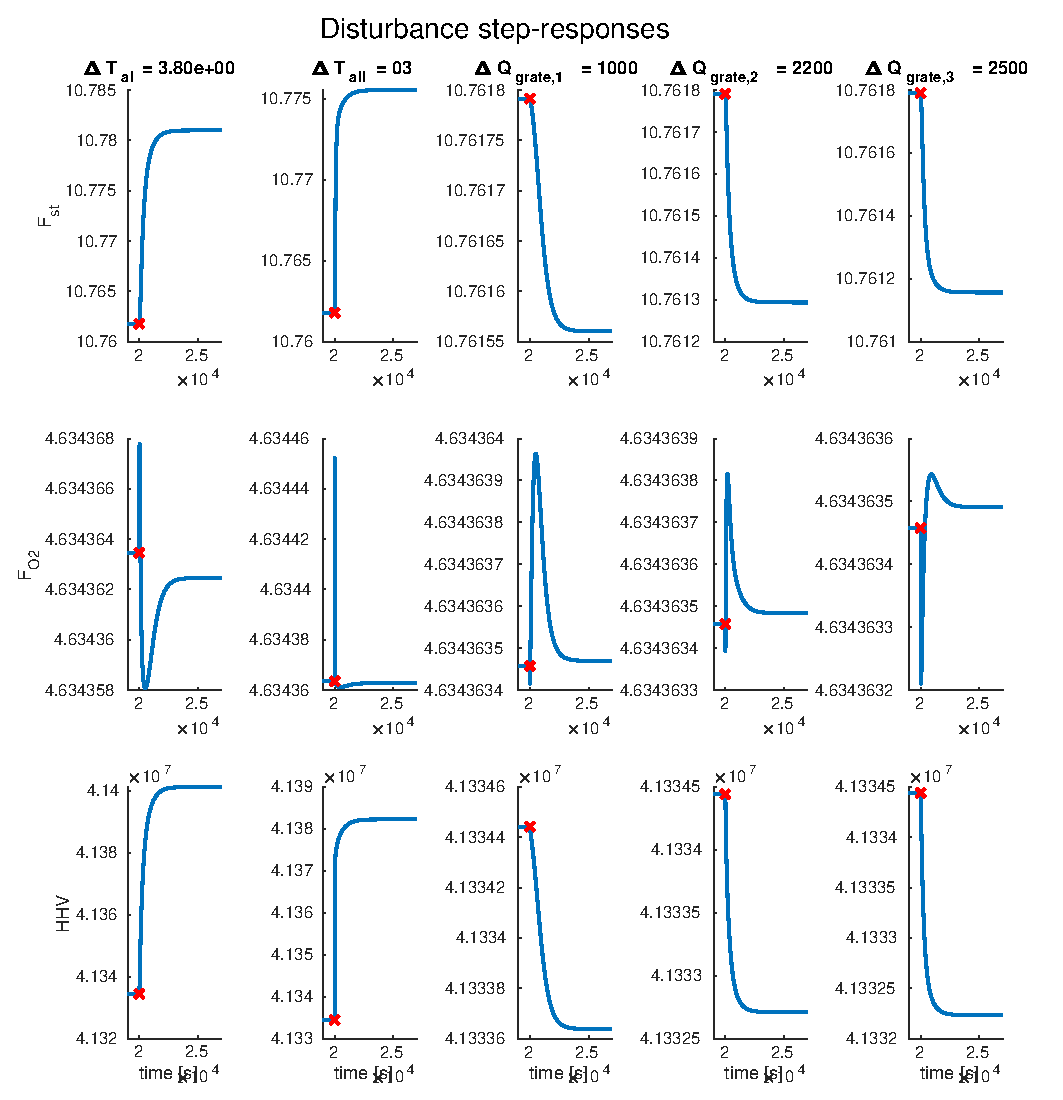
\includegraphics[width=\textwidth]{img/Simple_analysis_plots/Unscaled_disturbance_step_responses.eps}
    \caption{Step-response to the different kinds of disturbances}
    \label{fig:Unscaled_disturbance_response}
\end{figure}

The first two columns in figure \ref{fig:Unscaled_disturbance_response} show the effects of changes in the temperature of the primary and secondary air flow. The three different $Q_{\text{grate}}$ variables represent heat-exchange in the different sections of the grate. In practice, there should also be other variables as well, to represent sudden changes in the concentration of combustible materials or moisture in the waste. But the disturbances that are there show a few very interesting points. The first observation is the small effect that air-temperature has on the steam-production. Figure \ref{fig:Scaled_disturbance_response} show that a change of one degree in the temperature of the primary or secondary air will only change the steam-production by $4 \left[ \frac{kg}{s} \right]$. On the other had, the three values for $Q_{\text{grate}}$ fluctuate more in the range of $10^4$, so all changes in air temperature become completely dominated by the disturbances from $Q_{\text{grate}}$. Because of this, the disturbances resulting from changes in air temperature will not be taken into consideration when designing controllers.
\todo[inline]{Should there be another form of disturbance instead?}
\noindent
Finally, the biggest takeaway from plotting the disturbances can be seen when looking at the effects both of them have on $F_{O2}$. As a result, the disturbances almost entirely affect the production of steam, while most changes to the mass-flow of air in the flue gas are a result of the attempts to correct the disturbances. This means that a feed-forward controller that tries to cancel the effects of $Q_{\text{grate}}$ can only focus on the steam-production, and then another feed forward controller can be used to negate the changes in $F_{O2}$ that result from trying to correct for the changes in $F_{st}$


\noindent

\todo[inline]{Add this section}

\begin{figure}[!ht]
    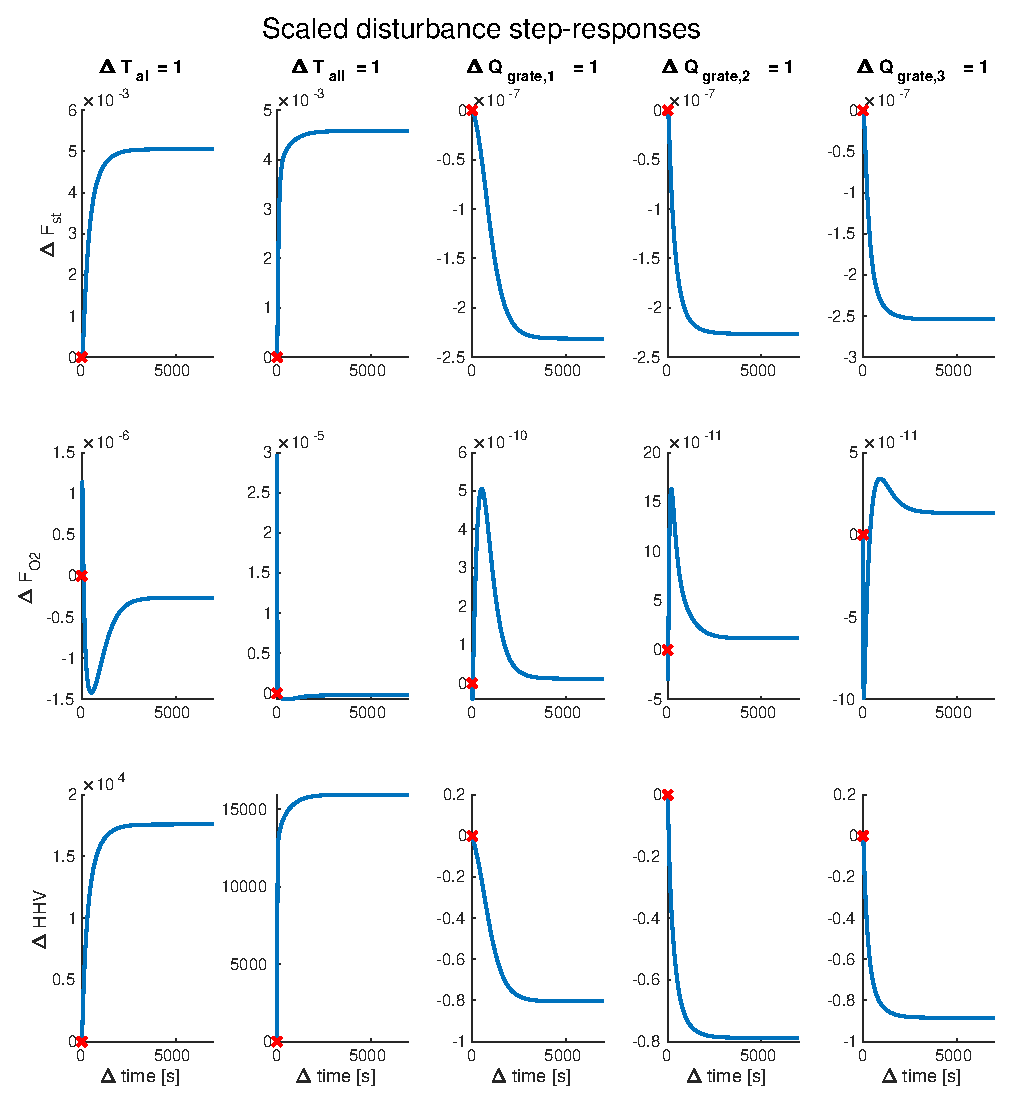
\includegraphics[width=\textwidth]{img/Simple_analysis_plots/Scaled_disturbance_step_responses.eps}
    \caption{Change in outputs, given step-changes in the the disturbances. Adjusted for the operating point, and scaled for the step-amplitude}
    \label{fig:Scaled_disturbance_response}
\end{figure}
\todo[inline]{Add units to the plots. Oxygen is [?/s], while HHV is [J/s]}



\section{Some observations}

\subsection{Justifying the use of an HHV-estimator}

When looking at figures \ref{fig:unscaled_Input_step_response} and \ref{fig:Unscaled_disturbance_response}, it can be seen that $F_{st}$ and $\hat{HHV}$ are remarkably similair, except for their amplitude. Since $F_{st}$ is one of the controlled outputs, the question becomes why $\hat{HHV}$ is necessary. 
\begin{figure}[!ht]
    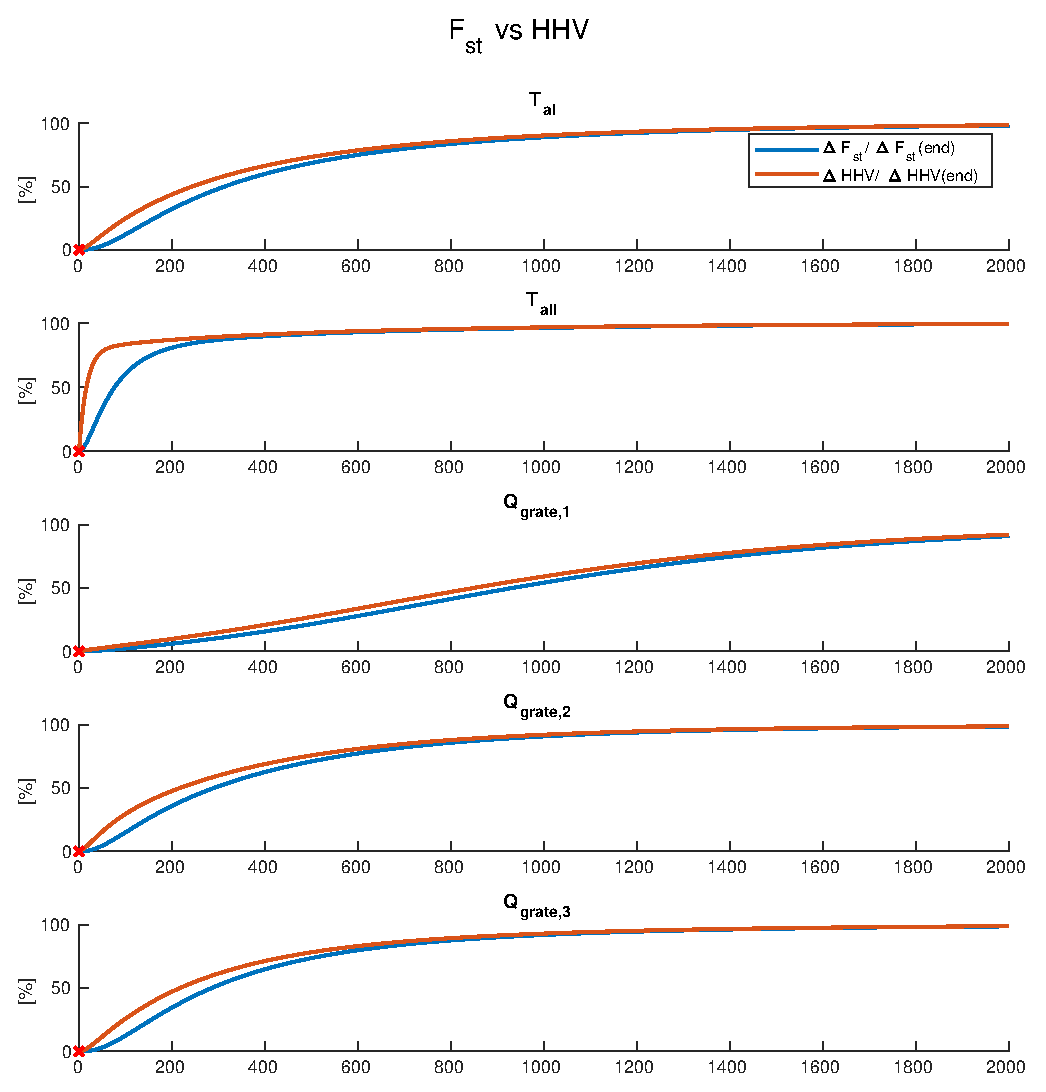
\includegraphics[width=\textwidth]{img/Simple_analysis_plots/Compare_F_st_to_HHV.eps}
    \caption{Change in $\hat{HHV}$ and $F_{st}$ as percentage of total change. Given as percentage to make them comparable.}
    \label{fig:F_st_vs_HHV}
\end{figure}
\noindent
Figure \ref{fig:F_st_vs_HHV} shows the step-responses of  $F_{st}$ and $\hat{HHV}$, without the mean, and represented as percentage of the infinite-horizon change. The two plots are very similair, but $F_{st}$ lags behind $\hat{HHV}$ by about a minute. In the case of PID-controller, this opens up for using a cascaded PID-controller, as was done in \cite{summer_student}, which allows for higher bandwidht, while also keeping the robustness of the previous controller. A model-based controller will be able to use the extra measurement of $\hat{HHV}$ to detect any changes in plant-disturbances earlier, but also to as a means to mitigate the effects of measurement-noise, as long as the two measurements are uncorrolated. 

\subsection{Usage of air when controlling steam production}

The results that will be discussed in section \ref{sec:MPC_results} show that some controllers will attempt to primarily use air to control the steam-production around the operating point. This is normally bad, but the way it is done is somewhat interesting. Instead of using $F_{aI}$, like it has been done in the previous controllers, it instead uses $F_{aI} -F_{aII}$ to increase the production of steam. There are two main reasons for doing this. Primarily, because changing $F_{aI}$ - $F_{aII}$  does not affect the total amount of oxygen added to the flue gas, leading to fewer changes in $F_{O2}$. The second reason can be seen in figure \ref{fig:F_diff_impulse_response}. By keeping the total amount of oxygen injected into the system constant, the step-response becomes more well-behaved, potentially leading to a controller that can be allowed to be more aggressive. 



\begin{figure}[!ht]
    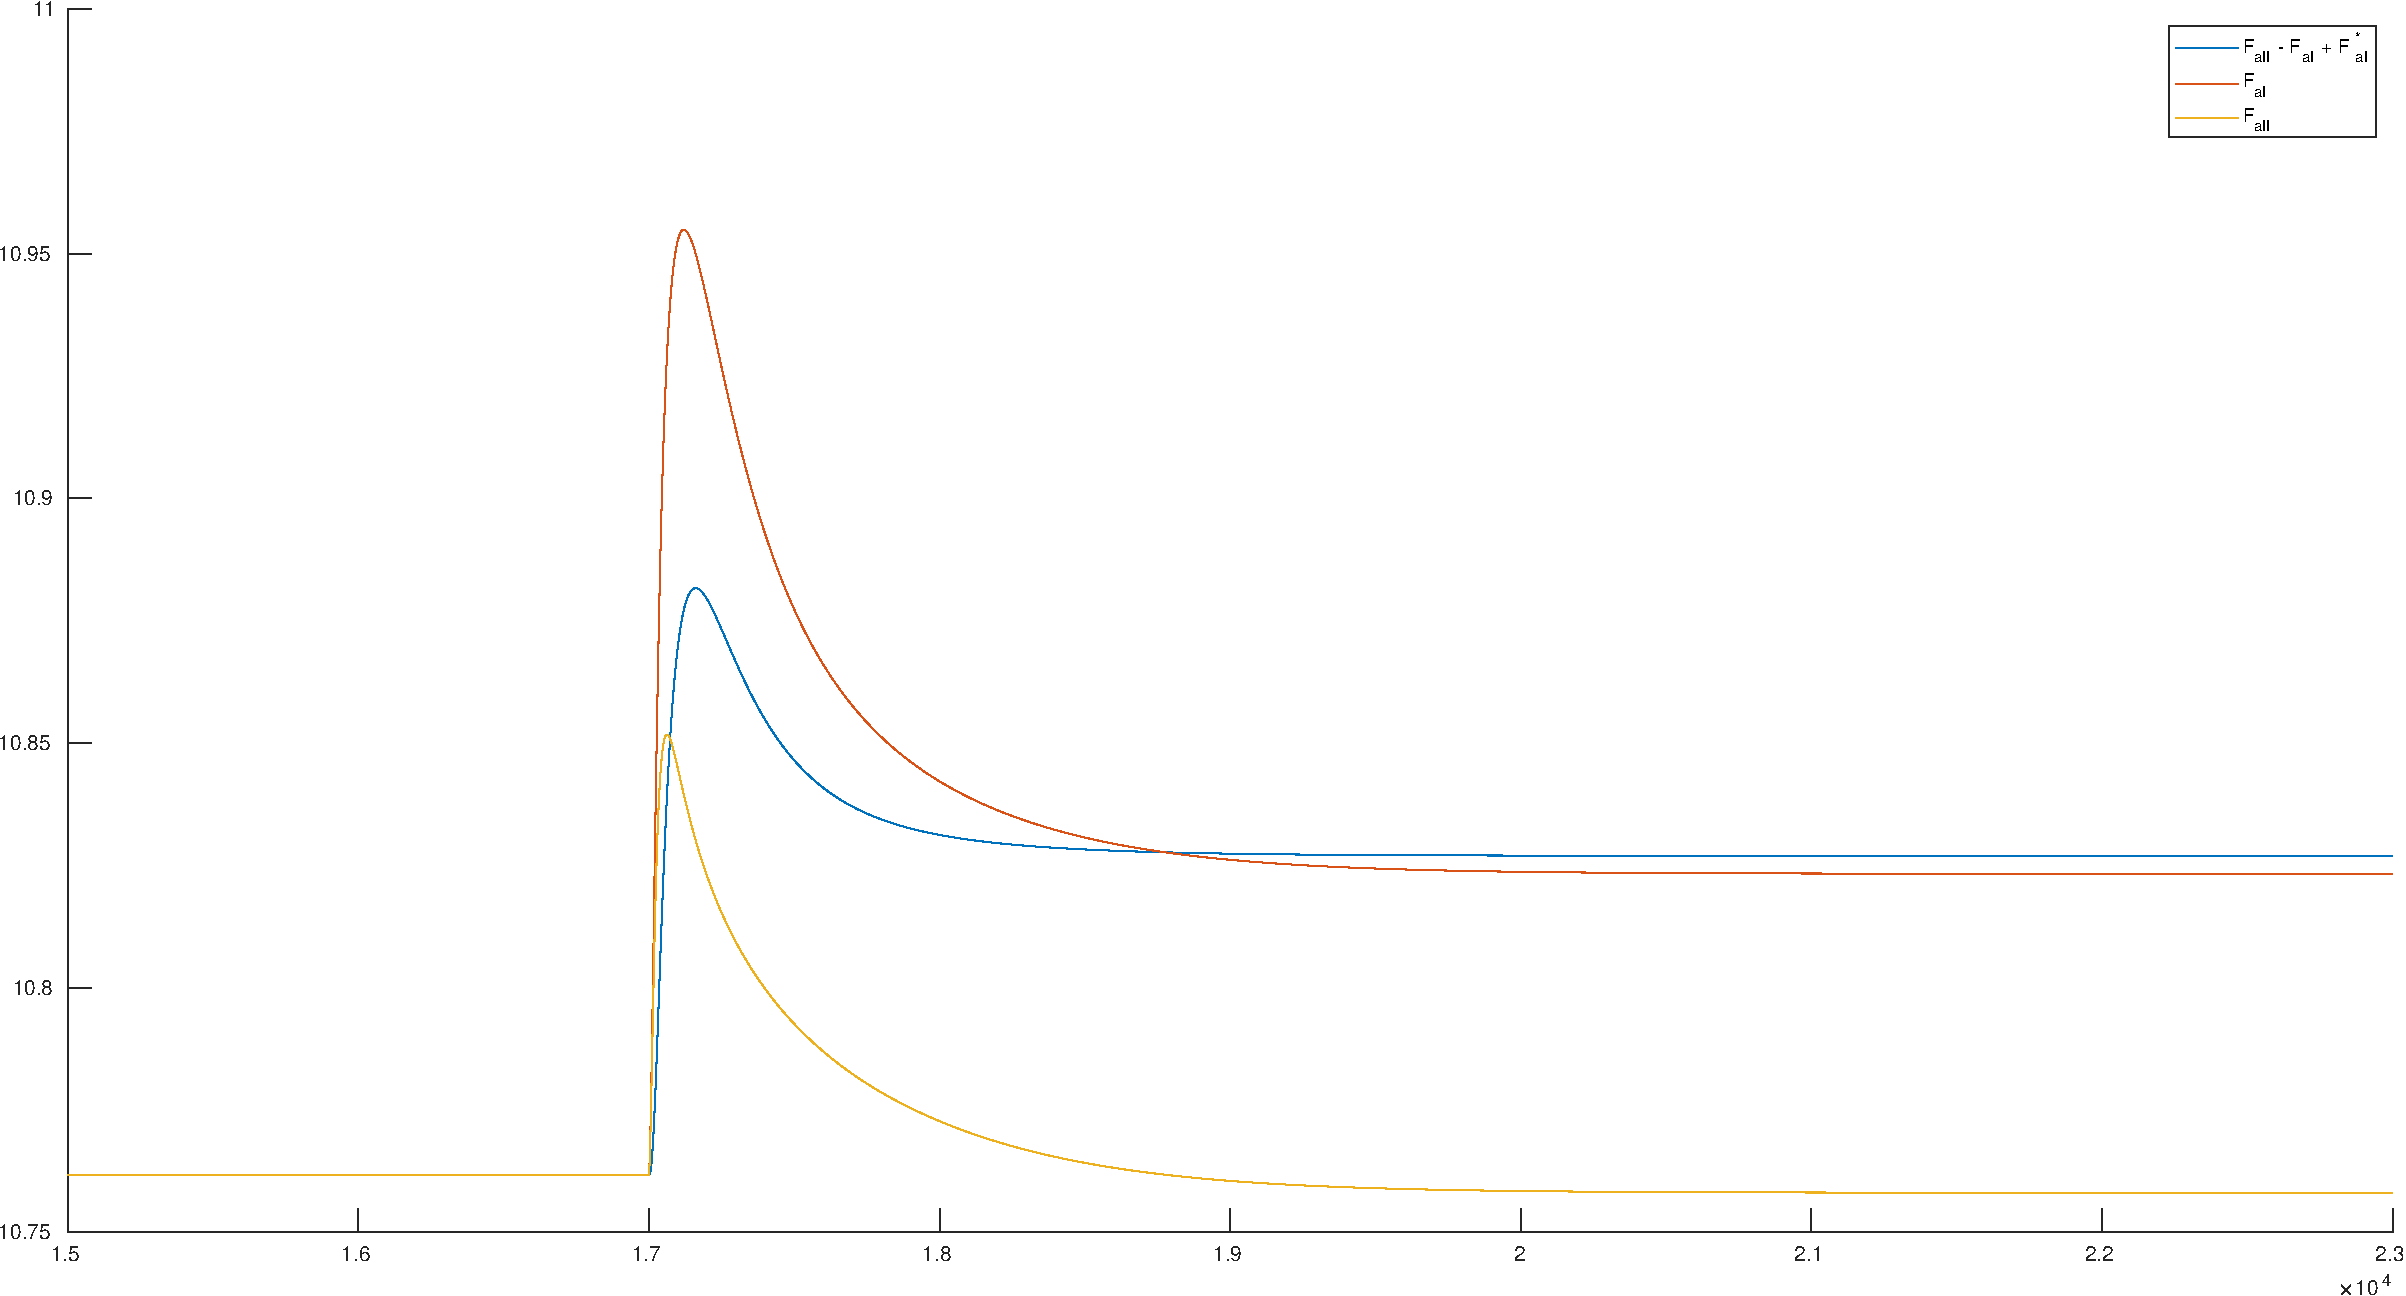
\includegraphics[width=\textwidth]{img/compare_steam_from_air_inputs-eps-converted-to.pdf}
    \caption{Change in outputs, given step-changes in the the disturbances. Adjusted for the operating point, and scaled for the step-amplitude}
    \label{fig:F_diff_impulse_response}
\end{figure}

A PID-controller with this premise was not implemented in this project, but it could potentially be an avenue for further research. 
\todo[inline]{Add this section @@@}

\chapter{Parameter estimation}
\label{sec:ERA}

Even if most physical constants are known, there are always some that are specific for each plant. They have to be measured or estimated, since they can be dependant on properties unique to each plant, like size, mass, etc. There are be methods for estimating the dynamics of nonlinear plants, but linear approximations are often much easier to perform, and has well-known methods that can be used without full state measurement. As long as the plant is sufficiently well-behaved and the state remains close enough to the operating point linear parameter estimation is preferred. 

\noindent
There are several robust methods for approximating the parameters of MISO systems or MIMO-systems where the outputs are loosely coupled, as shown in \cite{Adaptiv_boken}. But, in the case of the MSWC-plant, the fact that the amount of oxygen consumed in the and the amount of heat produced makes it steam somewhat unreasonable that these two output variables should be independent. As a result, a MIMO-scheme for parameter estimation is needed instead. There are several different methods of performing linear parameter estimation, like the state-space approach and a transfer-function based approach, as presented in \cite{MIMO_estimation}. However, in this project, the Eigensystem Realisation Algorithm (ERA) was used instead. This is mostly because it can estimate systems without full-state measurement. Additionally, the fact that it is somewhat easier to understand and implement made it the preferred candidate for parameter estimation. 


\section{Eigensystem Realisation Algorithm}
The ERA, as described in \cite{ERA_source}, is a method for estimating linear, discrete systems when the impulse response is known for some measurements of a system.  It also allows for the creation of reduced-order models, that describe the dominant dynamics of the impulse-response, even if the original system was of a higher order than the estimated one. 

The ERA assumes that the system is linear on the form:
\begin{align}
    \vec{x}_{k+1} &= A \vec{x}_k + B \vec{u}_k  \\
    \vec{y}_k &= C \vec{x}_k + D \vec{x}_u
\end{align}

Where 
\begin{align*}
    x \in \Re^n \\
    u \in \Re^m \\
    y \in \Re^p \\
\end{align*}
\noindent
$y$ and $u$ must be measured, but the states $x$ can be unknown. Unless full-state measurement is available, the states $x$ in the estimated system will correspond to some abstract values that do not need to correspond to any of the physical states of the real plant. The ERA is based on the impulse-responses of the discrete system. It uses the impulse-response from each separate input. If $\vec{u}_{0,i}$ is a Kronecker delta at element $i$ and 0 everywhere else, then the impulse-response $y_i$ for that input can be written as:

\begin{align}
    y_{0,i} &= D \vec{u}_{0,i} \\
    y_{k,i} &= C A^{k-1} B \vec{u}_{0,i} \forall k = 1,2,...
    \label{eq:impulse_dynamics}
\end{align}

All possible impulse-responses at one time-step can be combined into one matrix $Y_{k}$. 
\begin{align}
    Y_{k} = 
    \begin{bmatrix}
        y_{k,1} & y_{k,2} & \dots & y_{k,m}
    \end{bmatrix}
\end{align}


\noindent

The concatenation of all input-vectors $u_{k,i}$ is the same as 
\begin{align}
    I = \begin{bmatrix} u_{0,1} & u_{0,2} & \cdots & u_{0,m} \end{bmatrix}    
    \label{eq:impulse_structure}
\end{align}

By combining equation \ref{eq:impulse_dynamics} and \ref{eq:impulse_structure}, $Y_{k}$ can be written quite conveniently as a matrix-product. 
\begin{align}
    Y_{k} = C A^{k-1} B
\end{align}
All the impulse responses can be written into a $r \times s$ block matrix, on the form of a Hankel -matrix. 

\begin{align}
    H_k = \begin{bmatrix}
        \vec{Y}_{k+1} & \vec{Y}_{k+2} & \dots & \vec{Y}_{k+s}\\ 
        \vec{Y}_{k+2} & \vec{Y}_{k+3} & \dots & \vec{Y}_{k+s+1}\\
        \vdots & \vdots & \ddots & \vdots\\
        \vec{Y}_{k+r} & \vec{Y}_{k+r+1} & \dots & \vec{Y}_{k+r+s}
    \end{bmatrix}
\end{align}
This also means that the Hankel-matrix can ideally also be expressed by using $\left[ A,B,C \right]$. For instance The first matrix, $H_1$ can be written as: 

\begin{align}
    H_1 = 
    \begin{bmatrix}
        CB & CAB & \dots & CA^{m-1}B\\ 
        CAB & CA^2B & \dots & CA^{m}B\\
        \vdots & \vdots & \ddots & \vdots\\
        CA^{m-1}B & CA^{m}B & \dots & CA^{2m-2}B
    \end{bmatrix} 
\end{align}
 
\noindent
$H_1$ can equivalently be written as $H_1 = \mathbb{O}\mathbb{C}$, which is the product of the adjoint impulse response $\mathbb{O}$ and the direct impulse response matrix $\mathbb{C}$. These are given by:

\begin{align}
\mathbb{O} = 
\begin{bmatrix}
    C \\ CA \\ CA^2 \\ \vdots \\ CA^{m-1}
\end{bmatrix}
\vec{u}_0
\end{align}

\begin{align}
\mathbb{C} = 
\begin{bmatrix}
    B & AB& \dots & A^{m-1}B
\end{bmatrix}                             
\end{align}
The matrices $\mathbb{O}$ and $\mathbb{C}$ are also the same as the observability matrix and the controllability matrix. Any following matrix $H_k$ can be described as $H_k = \mathbb{O}A^k \mathbb{C}$.
Since $A$, $B$ and $C$ are unknown, the goal is to find some matrices $\hat{A}$, $\hat{B}$ and $\hat{C}$ which is able to produce the same (Or a similar) Hankel-matrix.  

\noindent
$Y_{k+1}$ can be extracted quite easily from $H_k$. If the matrix $E_p^T = \left[ I_p, 0_p, \dots, 0_p \right]$ and $E_m^T = \left[ I_m, 0_m, \dots, 0_m \right]$, then 
\begin{align}
    Y_{k+1} = E_p H_k E_m = E_p \mathbb{O}  A^k \mathbb{C}  E_m
    \label{eq:magic_eq_1}
\end{align}
This structure will be used to find good good matrices $\hat{A}$, $\hat{B}$ and $\hat{C}$. 
\noindent
In \cite{ERA_source} a matrix $H^\#$ is found, which has the properties 
\begin{align}
    \mathbb{O} H^\# \mathbb{C} = I_n 
    \label{eq:H_sharp_cancelation}
\end{align}
The matrix $H^\#$ satisfies being the pseudoinverse of $H_1$, but we will not prove that in this thesis.
\noindent
Another important tool will be the Singular Value Decomposition (SVD) of $H_1$


\begin{align}
    H_1 = U \Sigma V^*  
\end{align}

\noindent
The SVD has the property that all the column vectors in the matrices $U$ and $V$ are orthonormal to the other vectors from the same matrix. This is because the Hankel-matrix is purely real. This means that $VV^*=I$ and $U^TU=I$. $\Sigma$ is a diagonal matrix of positive elements.
Finally, we introduce the matrices $U_d$ and $U_d^\#$
\begin{align}
    U_d &= U \Sigma \\
    U_d ^\# &= \Sigma^{-1}U^T
\end{align}

\cite{ERA_source} also shows that $H^\# = VU^\#_d $. By inserting equation \ref{eq:H_sharp_cancelation} into equation \ref{eq:magic_eq_1}, a new expression can be found. 

\begin{align}
    \label{eq:magic_eq_2}
    Y_{k+1} = E_p \mathbb{O} \mathbb{C}H^\#  \mathbb{O} A^k \mathbb{C}H^\#  \mathbb{O}\mathbb{C}  E_m
\end{align}

Next, $\mathbb{O}\mathbb{C}$ can be contracted, and $H^\# $ can be replaced by $VU_d^\#$. 
\begin{align}
    Y_{k+1} = E_p H_1 V U_d^\#  \mathbb{O} A^k \mathbb{C} V U_d^\# H_1  E_m
\end{align}
Next, a trick is needed to get rid of the expression containing $A^k$. To use this trick, we will have to show that $\left[ U_d^\# H_2 V\right]^k  = \left[ U_d^\# \mathbb{O} A \mathbb{C} V \right]^k $ is the same as $U_d^\#  \mathbb{O} A^k \mathbb{C} V$. A polynomial $\left[ U_d^\# \mathbb{O} A \mathbb{C} V\right]^k$ can be written as $(U_d^\# \mathbb{O} A \mathbb{C} V)...(U_d^\# \mathbb{O} A \mathbb{C} V)$. By opening the parenthesis and replacing $VU_d^\#$ with $H^\#$, and then replacing any $\mathbb{C}H^\#\mathbb{O}$ with $I_p$, the result is $ = U_d^\# \mathbb{O}( A I_p)^k \mathbb{C} V$. As a result the two expressions are the same and equation \ref{eq:magic_eq_2} can be rewritten as: 
\begin{align}
    Y_{k+1} = E_pH_1 V \left[ U_d^\# H_2 V\right]^k  U_d^\# H_1  E_m
\end{align}

Finally, since $U_d^\# = \Sigma^{-1} U^T$, the square root of $\Sigma$ can be taken, and extracted from the exponential term, giving 

\begin{align}
    Y_{k+1} = E_p U \Sigma^{\frac{1}{2}} \left[ \Sigma^{-\frac{1}{2}} U^T H_2 V \Sigma^{-\frac{1}{2}} \right]^k \Sigma^{\frac{1}{2}} V^T E_m
\end{align}

This final equation gives a formulation that makes it possible to extract estimates of $A$, $B$ and $C$ that will have the same impulse-response. We will denote these estimates with a symbol hat. 
\begin{align}
    \hat{A} &= \Sigma^{-\frac{1}{2}} U^T H_2 V \Sigma^{-\frac{1}{2}} \\
    \hat{B} &= \Sigma^{\frac{1}{2}} V^T E_m \\
    \hat{C} &= E_p U \Sigma^{\frac{1}{2}}  \\
\end{align}


\noindent
Under idealised circumstances, the rank of the Hankel-matrix can be found when performing the SVD, as all elements after a given index will be 0. As a result, it will not matter if $\Sigma$, $U$ and $V$ are all truncated after that given index. The matrices can be divided into two parts. The part that is used to estimate the system, and the part that can be truncated. 

\begin{align}
    \Sigma = 
    \begin{bmatrix}
        \tilde{\Sigma} & 0 \\
        0 & \Sigma_{tr}
    \end{bmatrix}\\
    U = 
    \begin{bmatrix}
        \tilde{U} & U_{tr}
    \end{bmatrix}\\
    V = 
    \begin{bmatrix}
        \tilde{V} & V_{tr}
    \end{bmatrix}\\
\end{align}

If all sub-matrices with subscript tr truly are equal to 0, then 
\begin{align}
    U\Sigma V^* = \tilde{U}\tilde{\Sigma}\tilde{V}^*
\end{align}
\noindent
Consequently, the truncated matrices can be used to find a minimal representation of $\left[ \hat{A}, \hat{B}, \hat{C} \right]$. In reality, noise, non-linearities, and numerical errors are inevitable, so the rank of the Hankel-matrix can not be given certainly. Furthermore, in the case of this project, it will be highly desirable to have a model of reduced order, since it will speed up an MPC-controller significantly. 
\noindent
So, in practice, some index is simply chosen for where to cut off $\tilde{\Sigma}$. A common way to find a decent index is to choose some value $\epsilon$, such that 

\begin{align}
    \frac{\text{sum(diag(}\tilde{\Sigma}))}{\text{sum(diag(}\Sigma))} \ge \left( 1 - \epsilon \right)
\end{align}
And then making $\tilde{\Sigma}$ to be as small as possible, while satisfying the condition. By plotting the values of $\tilde{\Sigma}$, it also becomes a lot easier to see what is to be gained by adding more states to the estimated model. 
\todo[inline]{Add a figure of how this is done}

\noindent
Finally, it is important to remark that unless all states are observed, the states that result from the SVD will not necessarily represent physical values, but rather some linear combination of underlying properties of the system. This can easily be proven.
\noindent
For any non-singular matrix T, the triplet $\left[TAT^{-1}, TB, CT^{-1}\right]$ will result in the same Hankel-matrix as $\left[ A,B,C \right]$
\begin{align}
    CT^{-1} \left( TAT^{-1} \right)^k TB = CA^kB
\end{align}
This means that any true system representing a physical process can be transformed into infinitely many other systems that will have the same input-output response. 



\subsection{Handling Hysteresis}
If the system suffers from a small amount of hysteresis, or nonlinearities at the at first when responding to an impulse, then the impulse-response of the physical system may not reflect the dynamics of the linearized system very well. The solution to this is to use some kind of more permanent excitation, and then using that to find some other kind of excitation and then using that to get an estimate of what the impulse-response would have been without the transient nonlinearities. The normal method is to use Observer Kalman Filter Identification (OKID) to find out what the impulse-response "would have been" for a linear system, given some pseudorandom input. The asymptotic memory-usage of OKID is $O(n^2)$, so if the number of samples is too large, the required space needed for system identification will be several gigabytes. In those cases, a simple trick with the step-response can be used instead. If a linear model should be valid, then the principle of superposition should also be somewhat true. This means that the response $y$ from a sum  of inputs and initial sates is the same as the sum of the responses that would have resulted from each separate signal. 

\begin{align}
    y(u_1 + u_2) = y(u_1) + y(u_2) \\
    \alpha y(u) = y(\alpha u)
\end{align}

An impulse is just two step-inputs subtracted by each other if they have the same amplitude, but different delay.
\begin{align}
    \delta(T_i) = u(T_i) - u(T_{i-1})
\end{align}

Therefore, the superposition-principle allows us to find the impulse-response by subtracting a step-response by a delayed version of itself. 

If the plant is asymptotically BIBO (Bounded Input, Bounded output)-stable, then this allows us to avoid some of the issues related to hysteresis, or nonlinearities at the beginning of a response. 






\chapter{Controllers}
\label{cha:controllers}
There are several methods for controlling multivariable systems. While basic PID-controllers or linear controllers may be employed, it may in some cases be more useful to use a controller that allows the user to prioritize certain control variables, as well as enforcing strict or semi-strict limits on both inputs and states. Since there are strict limits that dictate a minimum oxygen concentration in the flue gas, a Model Predictive Controller (MPC) will be tested in this project.



\section{Model Predictive Control}
\label{sec:MPC}

The main idea of an MPC is that it contains some kind of model of the process that it is supposed to control. If we let $\vec{x}$ be a vector denoting the state of a system, $\vec{u}$ its input and $\vec{d}$ the disturbances, a model can be written as:

\begin{align}
  \vec{x}_{k+1}   = f_K\left( \vec{x}_{k} , \vec{u}_k , \vec{d}_{disturbance,k} \right)
  \forall k \in \left[ T_0, ..., T_n \right]
\end{align}

\noindent
Where $k$ represents all time-steps from the current time-step $T_0$ to some prediction horizon $T_n$ that may be defined by the one who makes the MPC. Even though the system is discretized, it is not required that an MPC has a uniform length between each time-step. As a result, each equation $f_k$ can be different, if there is a need for higher resolution at a shorter time-horizon. In this thesis, all time-steps will have the same length, so $f_i = f_j \forall i,j \in \left[ T_0,...,T_n] \right]$

On a similar form to $f$, the expected output from the system will be given by:
\begin{align}
  \vec{y}_k = g_K\left( \vec{x}_k, \vec{u}_k , \vec{d}_{noise, k} \right)
\end{align}

\noindent
The MPC always works on minimising some kind of objective function, that may take in a combination of inputs, outputs and states. as a result, it is necessary to make vectors containing all states in a prediction.
\begin{align}
  \vec{X} =
  \begin{bmatrix}
    \vec{x}_{T_0}^T & \vec{x}_{T_1}^T & \hdots & \vec{x}_{T_n}^T
  \end{bmatrix}^T \\
  \vec{U} =
  \begin{bmatrix}
    \vec{u}_{T_0}^T & \vec{u}_{T_1}^T & \hdots & \vec{u}_{T_n}^T
  \end{bmatrix}^T \\
  \vec{Y} =
  \begin{bmatrix}
    \vec{y}_{T_0}^T & \vec{y}_{T_1}^T & \hdots & \vec{y}_{T_n}^T
  \end{bmatrix}^T
\end{align}

\noindent
Finally, an MPC may also be under a set of equality constraints $h$ and inequality constraints $h$
\begin{align}
  g_i(\vec{X}, \vec{U}) \leq 0 \\
  h_i(\vec{X}, \vec{U}) = 0
\end{align}

\noindent
The constraints are normally only constraining the states or inputs at one time-step, but they can also be used to limit the rate of change of $\vec{u}_k$ or to lump together inputs if the MPC has a lower resolution closer to the prediction horizon.
\todo[inline]{Formulate better}

\noindent
If the function $V$ is used to describe the cost the MPC tries to minimise. The resulting problem becomes:
\begin{gather}
\begin{split}
  \text{min}_{\vec{U}} & V(\vec{X}, \vec{U}, \vec{Y})                                                      \\
  s.t                                                                                               \\
                & \vec{x}_{i+1} = f\left( \vec{x}_{k} , \vec{u}_k , \vec{d}_{disturbance,k} \right)\\
                & g_i(\vec{X}, \vec{U}) \leq 0  \forall i \in \left[ 1, \dots , N_{ieq} \right]     \\
                & h_i(\vec{X}, \vec{U}) = 0     \forall i \in \left[ 1, \dots , N_{eq} \right]      \\
  \end{split}
  \label{eq:generic_MPC_problem}
\end{gather}

\todo[inline]{This part should be written better}

\noindent
Equation \ref{eq:generic_MPC_problem} is quite generic and can represent a wide range of potential MPC-problems. Depending on the type of restriction that is set for the problem, more efficient algorithms may be used, which may speed up the speed of the MPC considerably. Because of the estimated model being linear, only linear MPCs will be considered in this thesis.



% \subsection{Nonlinear MPC}

% As was seen in Chapter \ref{cha:characteristics_of_process}, even the simplified model in \cite{waste_prof} has some nonlinearities in it. A priori, it will be somewhat difficult to say anything about how much these non-linearities will affect our ability to control the process. If no guarantees can be given for the operating point, it may be necessary to use a complex nonlinear MPC when optimizing the predicted system. A more complex model will take drastically longer to simulate and optimize, so this is something we want to avoid if possible.


% \noindent
% If a nonlinear problem is non-convex, it can become difficult to find a globally optimal solution through the use of iterative methods. This is because following a path from one local optimum to the global may require a solution to become temporarily worse. No proof is given that the control problem is of a convex form, but in \cite{waste_prof}, the problem was seemingly solved, partly by using simulated annealing, which can handle some non-convexity. If convexity can be guaranteed, then Sequential Quadratic Programming may be preferred. In this project, no non-linear model was found. Partly because of the complexity of the task, and partly because a linear model seemed serviceable and the biggest issues with the plant seemed to lie in how to effectively react to the disturbances while being affected by noise. 

\subsection{Linear MPC}



The Eigen-system Realisation Algorithm that was described in section \ref{sec:ERA} makes it possible to find a system representation from measured data. If such a model is combined with a Kalman-filter, it becomes possible to make a relatively fast model predictive controller. 

\noindent
The standard form for the problem that a linear MPC solves is on the form of a quadratic problem. Let m be the number of inputs and N is the number of prediction steps. H is a positive definite matrix $H \in \Re^{mN \times  mN}$ and F is some matrix $F \in \Re^{mN}$, while $U$ are all inputs over all timesteps within some prediction horizon, such that $\vec{U}\in \Re^{mN}$, then the problem can be described as: 

\begin{gather}
  \begin{split}    
  min_{\vec{U}} &       \vec{U}^T H\vec{U} + F\left( x_0, \text{ref}\right)^T \vec{U} \\
                & s.t:                                                                \\
                &       A_{ge} \vec{U} \geq b_{ge}                                    \\
                &       A_{eq} \vec{U} = b_{eq}                                       
  \end{split}
  \label{eq:linear_MPC_problem}
\end{gather}

\noindent
Unlike a lot of other model predictive controllers, the sequence of states $X$ can be implicitly expressed by a linear function of $x_0$ and the sequence of inputs $\vec{U}$. If the model is discrete, then the exact solution can be found by matrix-multiplications with a set of pre-prepared matrices. 

\begin{align}
  \vec{x}_{ T_{i+1}} = A\vec{x}_{ T_{i}}  + Bu_{ T_{i}}
\end{align}
Simply by adding all the inputs, and multiplying with A an apropriate ammount of times, a general expression can be found.
\begin{align}
  \vec{x}_{ T_{i} } = A^{i}\vec{x}_{ T_{0} }  + \sum_{j=1}^{i-1} A^{i-j}Bu_{T_{j}}
  \label{eq:multi_step_discrete_system}
\end{align}

\noindent
So if one matrix $\mathfrak{M}$ is constructed for the response due to the initial state $x_0$, and another one, $\mathfrak{C}$ for the convolution between the input signal and $A$, then all states in $\vec{X}$ can be represented by a few simple matrix operations

\begin{align}
  \vec{X} = \mathfrak{M} x_0 + \mathfrak{C} \vec{U}
\end{align}

\noindent
If $N$ is the number of time-steps that the MPC uses in its prediction, then the two matrices $\mathfrak{M}$ and $\mathfrak{C}$ are defined as:
\begin{align}
  \mathfrak{M} = \begin{bmatrix}
    A      \\
    A^2    \\
    \vdots \\
    A^{N}
  \end{bmatrix}
\end{align}

\begin{align}
  \mathfrak{C} =
  \begin{bmatrix}
    B        & 0        & \dots  & 0      & 0      \\
    AB       & B        & \dots  & 0      & 0      \\
    A^2B     & AB       & \dots  & 0      & 0      \\
    \vdots   & \vdots   & \ddots & \vdots & \vdots \\
    A^{N-2}B & A^{N-3}B & \dots  & B      & 0      \\
    A^{N-1}B & A^{N-2}B & \dots  & AB     & B      \\
  \end{bmatrix}
\end{align}
Because of this, any cost that would normally be written as a function the inputs and states can instead be expressed entirely by the inputs and the initial state. 
\begin{align}
  \vec{X}^T \hat{Q} \vec{X}
  = \left( \mathfrak{C}  \vec{U + \mathfrak{M}x_0}\right)^T \hat{Q} \left( \mathfrak{C}  \vec{U + \mathfrak{M}x_0}\right)
\end{align}

The same goes for constraints as well

\begin{align}
  A_{eq}\vec{X} = A_{eq}\left( \mathfrak{C}  \vec{U} + \mathfrak{M}x_0\right) \geq b_{eq} \\
  \Rightarrow A_{eq}\mathfrak{C}  \vec{U}  \geq b_{eq} - A_{eq}\mathfrak{M}x_0
\end{align}

Linear MPCs have the advantage of being able to use more efficient algorithms for solving the QP, than what would be possible for a generic non-linear problem. The result is that a faster sampling-frequency or longer prediction-horizons can be used. 

\subsection{Stabilizing an MPC}

A finite-horizon MPC is usually not guaranteed to stabilize a plant. Using a long prediction-horizon may solve this, but the number of prediction steps is dependant on the plant. Additionally, if the terminal state does not have a cost that reflects how the MPC will behave later, some strange behaviour might occur.  


\noindent 
Proof of unstability: Let $x\left[ T_{i+1} \right] = 2 \cdot x\left[ T_i \right] + u$ a scalar difference equation. If the cost-function is $J =x\left[ T_{i+1} \right]^2 + 3u^2$, simple differentiation gives that the best $u$ is $u = -\frac{1}{2} x\left[ T_i \right]$, which is not enough to stabilize the plant.


\noindent
As explained in appendix \ref{cha:LQR}, an LQR solves the same kind of problem an MPC does, but over an infinite horizon, and without constraints. If all constraints remain inactive  after the end of the prediction-horizon, and the terminal state-cost of the MPC is the same as the infinite-horizon state cost for the LQR, then the two controllers will have the exact same sequence of inputs. Since the LQR is guaranteed to stabilize the plant, the MPC will be guaranteed to do the same. 

\noindent
If only the state-feedback matrix $K_{\text{lqr}}$ is available, the infinite-horizon cost can be found by solving a Lyapunov-equation instead. 

\begin{align}
  \label{eq:Lyapunov_function}
  Q_{\infty} = (A-BK_{\text{lqr}})^T Q_{\infty} (A-BK_{\text{lqr}}) + Q_{\infty} + K_{\text{lqr}}^T R K_{\text{lqr}}
\end{align}
Luckily, Matlab implemented methods for solving both equation Lyapunov-equations and Riccati equations
\begin{align}
  K_{\text{lqr}} &= \text{lqr}\left(A,B,Q,R\right)\\
  Q_{\infty} &= \text{dlyap}((A-B*K_{\text{lqr}})^T, Q+K_{\text{lqr}}'*R*K_{\text{lqr}});
\end{align}

\subsection{Reference-tracking MPC}
MPC systems do not inherently track references. The way this is normally done is by giving a cost for changing the inputs, instead of using a cost for allowing the inputs to deviate from the reference point. This can the MPC to act differently from how the LQR that is used to make the infinite-horizon cost would have acted. One solution to stationary feed-forward input $v_{ff}$ that would cause the closed-loop system with and LQR.

\noindent
If an LQR is to track a reference, it usually means that the linearization point has to be changed. One way to solve this easily is to find a matrix that would cause the closed-loop LQR to converge assymptotically to the wanted output. If the closed loop is assymptotically stable, then the stationary output measurements can be found by: 
\begin{align}
  Y_{\infty} = C \left(I + BK -A \right)^{-1}B
\end{align}
It is possible to simply use the pseudoinverse of $\left(C \left(I + BK -A \right)^{-1}B\right)$ to find a matrix that can transform the set of desired outputs into the corresponding set of required inputs. A better solution can be found by solving a constrained QP \footnote{Quadratic Problem} that causes the reference to be tracked as cheaply as possible according to the original cost function. 
\begin{gather}
  \begin{split}
      min_{v_{ff}} & \left(\left( I +BK -A \right)^{-1} v_{ff}\right)^T \left(Q + K^T R K \right) \left( I + BK -A \right)^{-1}v_{ff} + v_{ff}^T R v_{ff} \\
      st:          &                                                                                                                                      \\
                  & C \left( I + BK - A  \right)^{-1} v_{ff} = y_{ref}                                                                                   
  \end{split}
\end{gather}
Additional constraints may be added if the problem is constrained. No proof was found in this thesis was would have allowed for tracking $y_{ref}$ as cheaply as possible without recalculating the QP each time the reference changes.
\todo[inline]{Check if this is true or not...}

\noindent
If the cost of the input-cost of an MPC is set to be given by $u - v_{ff}$, instead of $u$ and the state-cost is set to be given by $ x - \left( I + BK -A \right)^{-1}Bv_{ff}$, then the cost of the MPC will be zero when the system tracks the reference.

% \todo[inline]{Using PRBS with constant amplitude gives bias (?) "https://www.researchgate.net/post/Chirp_input_vs_Pseudo_Random_Binary_Signal---which_is_better_for_system_identification_of_a_Twin_Rotor_MIMO_SystemTRMS"}

% \todo[inline]{Iterating over one signal to excite at each time is usually also a bad idea since it introduces a bias}
\section{PID-control}


As has been seen in previous sections, it can be difficult to model the system. If it is possible to find a method that may control the plant, without having to rely on overly complex models or unreliable estimates, that would be desirable. Fortunately, normal cascaded PID-controllers can very often do an excellent job without an exact model. PID-controllers also often have the advantage of being robust against modelling errors. Unfortunately, tuning the three parameters in a PID-controller is known for being a difficult task, depending on the type of process. As a result, several different methods have been developed for tuning PID-controllers. This section will explain how to tune a PI or PID-controller by using Skogstad's Internal Mode Control (SIMC). 


\subsection{Skogstad's Internal Mode Control}

SIMC is a set of rules for tuning PID-controllers that were originally used for teaching-purposes, but who have proven to work very well in practice. The method is based, quite simply on exciting the system form a stationary state with a step-response. A step-response is often more well-behaved on most systems, and usually gives a response that is more in line with that of an actual linear system. The SIMC are the tuning rules for how to tune the constants of a PID-controller if a simple approximation of the model is already known. As a result, there are two parts of SIMC-tuning. The system approximation and the actual tuning. Because parts of the system are also affected by a rather large non-minimum phase response, it will also be necessary to expand upon the normal system approximation to handle the large transients. 





\subsection{Simplifying plant models}

Skogstad's method normally relies on some transfer function model of the system to tune the system. If $\tau$ represents the lag in the system and $e^{\theta_0 s}$ represents the delay and $k$ the plant gain, then Skogstad's method is based on a SISO (Single Input Single Output)  system that can be described as: 

\begin{align}
    y = k \cdot \frac{\prod_{i=1}^{n}  \left(  - T^{inv}_i s + 1\right)}{\prod_{j=1}^{n} \left( \tau_{j,0} s +1  \right)} e^{-\theta_{0} s}
\end{align}
Where $\tau_i \geq \tau_{i+1} \geq 0$ and $T^{inv}_i \geq T^{inv}_{i+1} \ge 0$ (Positive roots in the numerators are explained in subsection \ref{sec:positive_numerator_time_constants}). Since Skogstad's method only revolves around a PID-controller, only the most dominant terms are taken into consideration. Any factor after the second one will instead be approxomated by a the Taylor-approxomation of a time-delay and added to the already existing time-delay. 

\begin{align}
    e^{\tau_j s} &= 1 + \tau_j s + \dots \tau_j^i s^i + \dots &\approx 1 + \tau_j s \\
    e^{-\tau_j s} &= \frac{1}{e^{\tau_j s}} &\approx \frac{1}{\tau_j s +1}
\end{align}

\noindent
Depending on the properties of the plant, it is possible to perform different simplifications. If the lag $\tau_1$ dominates the process (usually $\tau_1 > 8\theta$), then the estimation $\frac{k}{\tau_1 s +1} \approx \frac{k'}{s}$ can be used. This can also alow you to end the experiment early instead of waiting for convergence. 
A discretely sampled with a sampling time $h$, can be simplified into a continuous system with an additional time-delay $\frac{h}{2}$  if the time-delay is not too dominant. Additionally, the largest neglected pole can be evenly distributed between the smallest lag that is being used and the time-delay.

\noindent 
All these rules can be summarized into the much simpler rules, described in equations \ref{eq:SIMC_approx_2nd_order} and \ref{eq:SIMC_approx_1st_order}. The tuning rules are lifted dirextly from equations (10) and (11) in \cite{SIMC_source}. 

\colorbox{gray}{\begin{minipage}{\textwidth}
    Second order approxomation :
\begin{align}
    \label{eq:SIMC_approx_2nd_order}
    \tau_1 = \tau_{1,0};&\tau_2 = \tau_{2,0} + \frac{ \tau_{3,0}}{2}; \theta = \theta_0 + \frac{\tau_{3,0}}{2} + \sum_{i \ge 4} \tau_{i,0} + \sum_j T^{inv}_{j0} \ \frac{h}{2}
\end{align}

First order approxomation: 
\begin{align}
    \label{eq:SIMC_approx_1st_order}
    \tau_1 = \tau_{1,0} + \frac{\tau_{2,0}}{2} ; \theta = \theta_0 + \frac{\tau_{2,0}}{2}  \sum_{i \ge 3} \tau_{i,0} + \sum_j T^{inv}_{j0} \ \frac{h}{2}
\end{align}
\end{minipage}}

\subsubsection{Positive time-constants in the numerator}
\label{sec:positive_numerator_time_constants}
In \cite{SIMC_source} positive roots in the numerator $\left( T_0 s +1 \right)$ are handled by allowing the term in the numerator to cancel one in the denominator (The closest, larger one). The delay $ \theta$ is the final delay after all cancellations have been made. Because of this, the cancellations have to be made iteratively with the new delays.

\begin{align}
    \frac{T_0 s +1}{\tau_0 s +1} \approx 
    \begin{cases}
        \frac{T_0}{\tau_0} & \text{if } T_0 \ge \tau_0 \ge \theta\\
        \frac{T_0}{\theta} & \text{if } T_0 \ge \theta \ge \tau_0\\
        1 & \text{if } \theta \ge T_0 \ge \tau_0\\
        \frac{T_0}{\tau_0} & \text{if } \tau_0 \ge T_0 \ge 5 \theta\\
        \frac{\left( \tilde{ \tau }_0 / \tau_0 \right)}{\left( \tilde{\tau}_0 - T_0  \right)s +1} & \text{if }  \tilde{\tau}_0 \delequal \text{min} \left( \tau_0, 5 \theta \right) \ge  T_0 
    \end{cases}
\end{align}
If there is no larger time-constant in the denominator, the closest smaller one is used instead. 

\subsection{PID-rules}
SIMC uses the IMC tuning rules for generating the PID-parameters after a first or second-order model has been found. A more complete derivation of the rules is found in \cite{SIMC_source}, but the short version is: 

\noindent
Usually, a desired response with time-constant $\tau_c$ is selected. $\tau_c$ is a tuning constant of the SIMC, that is the desired time-constant of the closed-loop system. 
\begin{align}
    \left(\frac{y}{y_{s}}\right)_{desired} = \frac{1}{\tau_c s +1} e^{\theta s}
\end{align}
 Let $g(s)$ be the transfer-function that describes the plant. An ideal controller $c^*(s)$ is choses such that if 
 \begin{align}
     g(s) = \frac{k}{\left( \tau_1 s+1 \right) \left( \tau_2 s +1 \right)} e^{\theta s}
 \end{align}
Then, the idealised controller can be writen as:
 \todo[inline]{I lef off correction here @@@}
 \begin{align}
    \frac{g(s) c^*(s)}{1 + g(s) c^*(s)} = \left(\frac{y}{y_{s}}\right)_{desired}
 \end{align}
\begin{align}
    c^*(s) = \frac{\left( \tau_1 s +1 \right)\left( \tau_2 s +1 \right)}{k} \frac{1}{\tau_c s+1 - e^{- \theta s}}
\end{align}
The Taylor-approxomation is used to get rid of the $e^{-\theta s} \approx 1 - \theta s$, such that the approxomated controller $c(s)$ becomes
\begin{align}
    \label{eq:delay_controller}
    c(s) = \frac{\left( \tau_1 s +1 \right)\left( \tau_2 s +1 \right)}{k} \frac{1}{\left( \tau_c + \theta \right)s}
\end{align}
becomes $ \left(\left( \tau_c + \theta \right)s\right)$. However, if the lag is the most dominant part of the process, this kind of tuning will result in a very slow setling-time.  This is solved by approximating the system as a pure integrating process with no $ \frac{k}{\tau_1 s +1 } e^{- \theta s} \approx \frac{k}{\tau_1 s} = \frac{k'}{s}$. Afterwards, $c(s)$ can be set as a PI-controller with gains that cause the closed loop to have a damping factor $\xi$ of 1
\begin{align}
    \label{eq:second_order_plant_feedback}
    \frac{g(s)c(s)}{1 + g(s)c(s)} = \frac{ \frac{k'}{s} K_c \left(1+ \frac{1}{\tau_I s}\right)}{1 + \frac{k'}{s} K_c \left(1+ \frac{1}{\tau_I s}\right)}
\end{align}
Sorting out the terms gives 
\begin{align}
    \frac{\tau_I s + 1}{\frac{\tau_I }{k' K_c}s^2 + \tau_I s + 1}
\end{align}

\noindent
A system on standard second order form is written as $\tau_0^2 s^2 + 2\tau_0 \xi s +1$. If $\xi =1$, any system with denominator on that form is critically damped. So, in the case of equation \ref{eq:second_order_plant_feedback}

\begin{align}
    \tau_0 = \sqrt{\frac{\tau_I}{k' K_c}}\\
    \xi = \frac{1}{2} \sqrt{k' K_c \tau_I}
\end{align}

\noindent
So if $K_c$  is chosen as in equation \ref{eq:delay_controller} to be $ \frac{1}{k} \frac{\tau_1}{\tau_c + \theta} $, then $\tau_I = 4\left(\tau_c + \theta \right)$. Both these tuning rules can be combined into one very simple one. 

\colorbox{gray}{\begin{minipage}{\textwidth}
\begin{align}
    \label{eq:SIMC_simple_tuning_rule}
    K_c     &= \frac{1}{k} \frac{\tau_1}{\tau_c + \theta}\\
    \tau_I  &= \text{min} \left\{ \tau_1, 4 \left( \tau_c + \theta \right)\right\}\\
    \tau_D  &= \tau_2
\end{align}
\end{minipage}}

\noindent
If a PI-controller is needed, a simpler model is used instead, such that $\tau_2 =0$. \cite{SIMC_source} mentions that $\tau_c \in [\theta , \infty)$ can be chosen freely, but that it is a tradeoff between speed and robustness (as well as smaller variations in inputs). The paper highlights that $\tau_c = \theta$ is a good tradeoff between speed and robustness. 


   



\subsection{PID-tuning by using bode-plots}


Although Skogstad's method can be very useful, it might sometimes struggle with systems where the poles or zeros are complex, since those cases are not defined in the original method. There are proposed methods for handling such cases, but it is also possible to simply tune a stable system by observing the phase-response of a stable system and choosing $K_{c}$ and $T_{I}$ such that a sufficient phase and gain margin can be achieved. If the system is stable and the controller is a simple PI-controller, then it is also possible to find a set of rules that can automate the tuning-process, so that it is robust against time-delays and modelling errors.

\subsubsection{A quick reintroduction to bode-plots (Nyquist's criteria of stability)}

Let the transfer-function of the plant be $h_p(s)$, and the transfer-function of the controller be $h_c(s)$. Let $h_0(s) = h_p(s) h_c(s)$ An instability in the system is caused if the transfer-function of the closed loop 

\begin{align}
    M(s) = \frac{h_0(s)}{1 + h_0(s)}
\end{align}
has a pole in the left half-plane. $1+ h_0(s)$ can be divided into a numerator and denominator, and the resulting closed-loop will have a set of poles and zeros 
\begin{align}
    1+ h_0(s) = 1 + \frac{n_0(s)}{d_0(s)} = \frac{d_0(s) + n_0(s)}{d_0(s)} = \frac{(s -\lambda_1) \dots ( s -\lambda_n)}{(s-\rho_1)\dots (s-\rho_n)}
\end{align}
If one performs integration of s along the imaginary axis, and then along a circle with an infinitely large radius in the right half-plane, only poles and zeros in the right half-plane will give a net contribution to the phase, as described in \cite{Regtek_boken}. This can be seen in figure \ref{fig:Nyquist_criteria}. All zeros $\lambda$ will give a net negative contribution to the angle, while all poles $\rho$ will give a positive contribution. 



\begin{figure}[h!]
    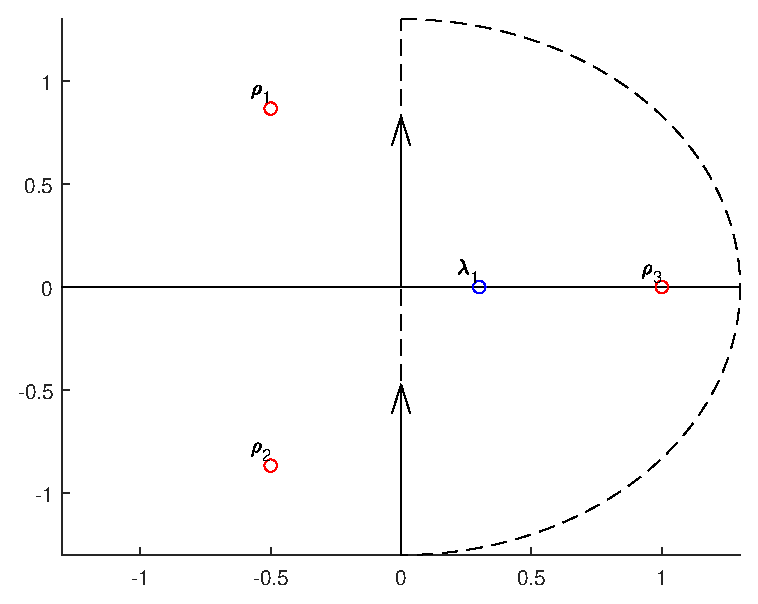
\includegraphics[width=\textwidth]{img/Fig_dump/Nyquist_criterion.eps}
    \caption{Poles $\rho$ and zeros $\lambda$ of a transfer-function. The existence of $\rho_3$ makes it unstable}
    \label{fig:Nyquist_criteria}
  \end{figure}

\noindent
$\Delta \angle (1 + h_0(s))$ is the total angular change when integrating along the half-circle. $N_p$ and $N_n$  are the total number of poles in the right half-plane in the open and closed system respectively. The resulting relation is 

\begin{align}
    \Delta \angle (1 + h_0(s)) = - 2\pi \left( N_n- N_p \right)
\end{align}
So, Nyquist's stability criteria uses the total phase-contribution of $1+h_0(s)$, and the number of unstable poles in the open-loop system to determine the number of unstable poles in the closed-loop 

\begin{align}
    N_n = N_p - \frac{\Delta \angle (1 + h_0(s))}{2\pi} 
    \label{eq:nequist_stability_criteria}
\end{align}
\noindent
To analyze if an open loop system will be stable when the loop is closed, a bode-plot, like in figure \ref{fig:generic_bode_plot} is normally used. A bode-plot consists of one plot of the amplitude of the open-loop, and the phase of the open-loop system. Both of them are plotted against an angular velocity, $\omega$.
\todo[inline]{Get figures that are cropped better }
\begin{figure}[ht]
    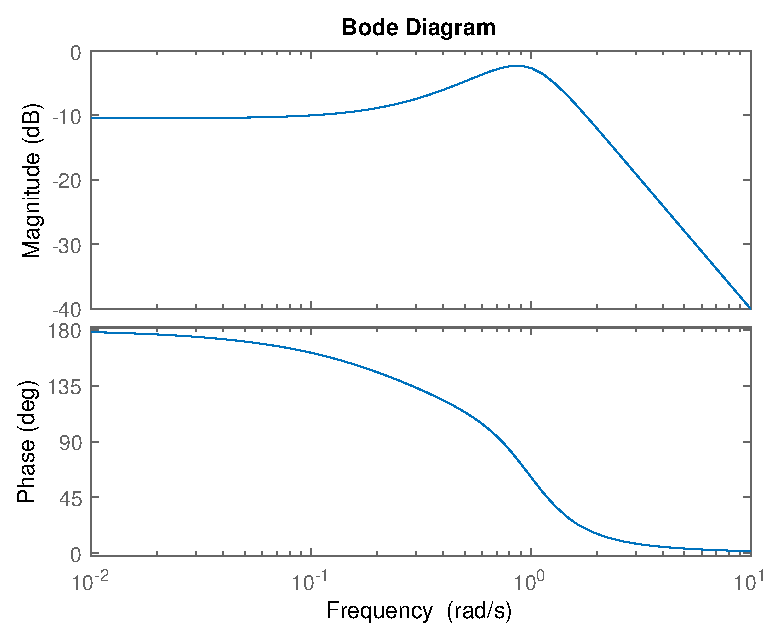
\includegraphics[width=\textwidth]{img/Fig_dump/Generic_bode_plot.eps}
    \caption{A generic bode-plot of $\frac{s-0.3}{s^2 + s + 1}$}.
    \label{fig:generic_bode_plot}
\end{figure}


\noindent
A bode-plot makes it very clear a stable system will be stable in a closed-loop as well. If the amplitude of $h_0(s)$ is greater than 1 (0 dB) when the phase is modulo 360 is -180 degrees, then the system is unstable. 



\subsection{Gain and phase margins of stable systems}


The plant that is being controlled is known to be stable, so the only condition that has to be satisfied is that the amplitude of the system is less than 0dB whenever the phase of the system crosses $-180^o$. It is never possible to know exactly how one might model the system incorrectly, but bode plots allow saying something about the robustness against time-delays and against unknown gains affecting the system. If a system has robustness in both of these regards, then it should also have some robustness to in regards to the modelling errors with regards to the system dynamics as well. 


\noindent
Since time-delays are written as $e^{\theta j \omega}$, they only contribute with an addition to the phase in the bode-plot. This means that a good phase-margin will give robustness against time-delays. Usually, it is said that a phase margin of $60^o$ and a gain margin of 20dB is a good balance between performance and robustness. 



\noindent

\subsubsection{Choosing a good controller}

One way to say something about a controller is by using the control ratio $N(s) = \frac{1}{1 + h_0(s)}$ and the following ratio $M(s) = \frac{h_0(s)}{1 + h_0(s)}$. $M$ tells how the system will track changing references of a given frequency, as a result, it will also say how much the system reacts to measurement noise. Meanwhile, N says how well noise or disturbance will be suppressed. When working with a system that is subject to both noise and process disturbances, both $N(s)$ and $M(s)$ are necessary. Ideally, $N(s)$ has such a shape that all disturbances become 0 while ignoring any noise. This is impossible, but it gives a hint as to how the controller and filters would be chosen. If it is known that some noise has a very specific frequency, then band-stop filters or notch-filters can be added to the controller as well. 
\begin{figure}[!ht]
    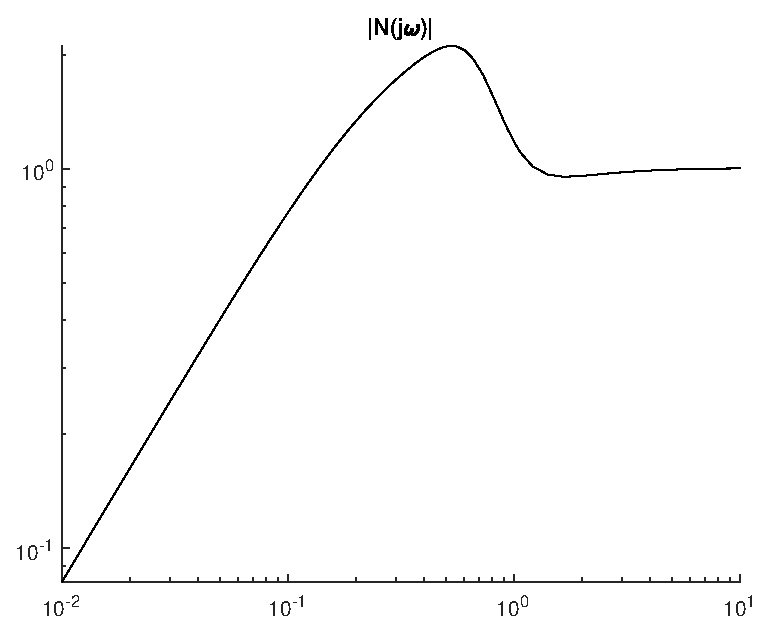
\includegraphics[width=\textwidth]{img/Fig_dump/Generic_N_plot.eps}
    \caption{N for a poorly controlled process}
    \label{fig:N_plot}
\end{figure}


\noindent
In figure \ref{fig:N_plot}, a plot of $N(j\omega)$ is given for some arbitrarily chosen controller. As can be seen in the plot, it does suppress disturbances at low frequencies. Additionally, it can be seen that for high frequences, the disturbances are simply let through. However, a rather large peak at around $0.3  \frac{rad}{s}$ can be seen as well. This peak around where the crossover-frequency, which means that $h_0(j\omega)$ almost entirely negative. As long as the phase of $h_0(j \omega)$ crosses $-180^o$, there is always a point where the amplitude of $N(j \omega) > 1$. The way to control the size of this peak is by making sure the amplitude of $h_0(s)$ is sufficiently small around $-180^o$, since if it were to be close to 1, then the system would amplify any noise or disturbance of that frequency by an almost absurd amount.


\noindent
There are two possible measures that can be taken to supress the resonance around the unwanted frequencies. The first is to simply increase the gain margin. If the amplitude of $h_o(j \omega)$ is small at $\angle h_o(j \omega) \approx -180$, then the fraction $\frac{1}{1 + h_0(j \omega)}$ does not grow as large. A phase margin of $20dB$ will ensure that the resonant amplitude will be less than $\frac{1}{1 - \frac{1}{10}} \approx 1.11$. 

\noindent
The second option is to use the D-part of the controller to "lift" the phase of the combined controller and plant. Normally, most plants attenuate high-frequency signals more than low-frequency ones, so by keeping the phase above $-180^o$ for longer, $|h_0(s)|$ can be made to be smaller at the new crossover frequency. Simply adding a differentiating term can sometimes lead to other problems, since it makes the system react more to high-frequency noise. The solution is to add a low-pass filter to the controller as well. An additional advantage of using a low-pass filter is that a differentiation term will usually require some numerical differentiation, that might be ill-behaved. A differentiation term in series with a low-pass filter gives a variation of a high-pass filter, which is a proper transfer function\footnote{Proper transfer function: The order of the denominator (Highest  degree of s) is greater or equal to the order of the numerator}, that can be written as a causal system and discretized in a more well-defined manner. 


\noindent

The need for low-pass filters can be shown in figure \ref{fig:M_plot}. Even if the plot for $N(s)$ looked good, $M(s)$ shows that high-frequency noise are not sufficiently attenuated, making it susceptible to noise, which is very often present in the form of electrical noise. 

\begin{figure}[!ht]
    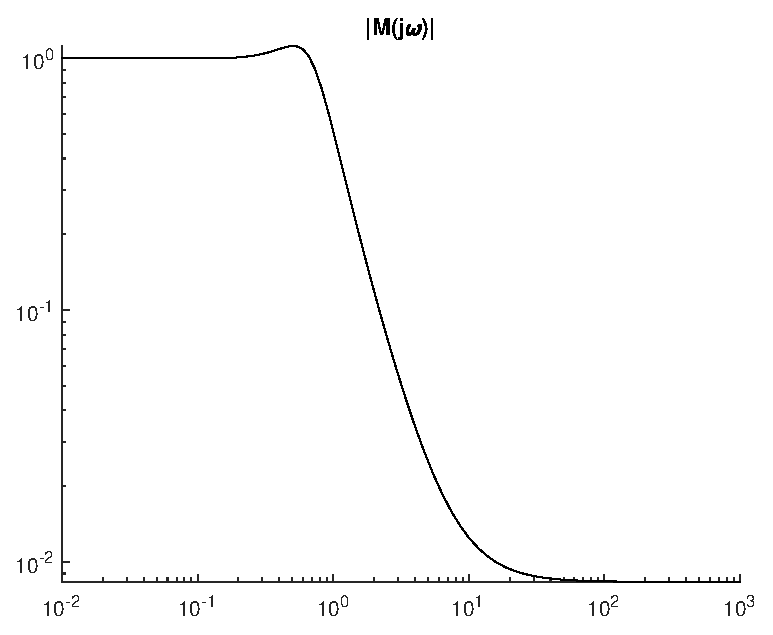
\includegraphics[width=\textwidth]{img/Fig_dump/Generic_M_plot.eps}
    \caption{M for a poorly controlled process}
    \label{fig:M_plot}
\end{figure}


\todo[inline]{I left off here}


% This can potentially be very bad if the system is subjected to the noise around those frequencies. The amplification of the noise is because of $h_0(j\omega)$ being almost purely negative and real at those frequencies. Preferably, $K_c$ should be chosen, such that $h_0(s)$ has a small amplitude when the phase is close to $-180$. This can be done by using a gain-margin that is sufficiently large. 



% Although we do not know the frequencies that make up the noise, it seems reasonable that there are patterns that happens hourly or daily (A change in quality, depending on the day, or if new waste is added roughly every hour). If a controller has terms that resonate around that frequency, then that is a bad choice for a controller. The good part about the controller is that $N(j\omega) \approx 1$ for all frequencies above $10^{-1}$ since the worst noise is most likely the disturbances that come from from the measurements in some form. 



\todo[inline]{Find the real names of M and N}







\chapter{Automated tuning}
\label{cha:automated_tuning}
The methods from Chapter \ref{cha:controllers} do not necessarily give controllers that work perfectly right away. Because of this, some manual tuning may be needed as well. Some of the required changes may be intuitive, while others may be dependant combinations of parameters, as well as some trial and error. As a result, the tuning process can be quite time-consuming. One solution to this is to make up some kind of measure of the quality of the system response, and then use an optimisation algorithm, like Nelder-Mead to minimise said cost.


\section{Nelder-mead}
The Nelder-Mead optimisation algorithm is a very popular method for optimising convex nonlinear problems. The main selling-point of Nelder-Mead is that the search of the optima is done entirely by a set of measured points and the corresponding values of the function, without the use of an approximated or an analytical gradient. This means that the algorithm tends to be a bit slower than most other optimisation algorithms, like SQP\footnote{SQP: Sequential Quadratic Programming}.Instead, it has the advantage of being usable on a wide set of convex functions without much prior knowledge about the function. It should be noted that according to \cite{Nelder_Mead_convergence_issues}, even though the algorithm works well in practice, it is possible for it to converge towards non-stationary points. 

\subsection{Theory}
\cite{Nelder_Mead_source} summarises the Nelder Mead algorithm quite nicely, so it will only be covered very briefly in this chapter. 

\noindent
Nelder-mead optimises an $N$-dimensional function by using a set $\mathbf{X} = \{x_1, x_{2}, \dots , x_{n+1}\}$ of $N+1$ points. The points are at all times sorted in such a way that
\begin{align}
    f(x_1) \leq f(x_2) \leq \dots \leq f(x_{n+1})
\end{align}

\noindent
At iteration k, the set $\mathbf{X}^k$ is updated to $\mathbf{X}^{k+1}$ by replacing the worst the worst point $x_{n+1}^k$ in the set. $x_{n+1}^k$ is reflected over or drawn to the "center of mass" $\Bar{x} = \sum_{i=1}^N\frac{x_i}{N}$ off the other points, depending on of it improves the point or not. The new point $x_{\text{new}}^k$ will be given by 

\begin{align}
    x_{\text{new}}^k = \Bar{x}^k + \rho (\Bar{x}^k - x_{n+1}^k) 
\end{align}
Several possible candidates along the line are tested. If the function $g^k(\cdot)$ is defined as 

\begin{align}
    g^k(\rho) = f( \Bar{x}^k + \rho (\Bar{x}^k - x_{n+1}^k)  )
\end{align}

\noindent
the update-rule for a single iteration is described in algorithm \ref{alg:update_simplex}. 
\begin{algorithm}
\label{alg:update_simplex}
\caption{Find $x_{\text{new}}^k = \Bar{x} + \rho(\Bar{x}^k - x^k_{n+1})$}
\begin{algorithmic}
\REQUIRE $x^k_{n+1} $, $\Bar{x}^k$, $g^k(\cdot)$, $f(x^k_{n+1})$
\ENSURE $y = x^n$
\IF{$g(1) < f(x^k_{n+1})$}
    \IF{$g(2) < g(1)$}
        \STATE $\rho =2$
    \ELSE
        \STATE $\rho = 1$
    \ENDIF
\ELSIF{ $g(1/2) < f(x^k_{n+1})$}
        \STATE $\rho =1/2$
\ELSE 
    \STATE $\rho = -1/2$
\ENDIF
\end{algorithmic}
\end{algorithm}


Afterwards, the new set $\mathbf{X}^{k+1}$ is given by 
\begin{align}
    \mathbf{X}^{k+1} = \{x^k_1,x^k_2, \cdots, x^k_n \} \cup \{x_{\text{new}}^k \}
\end{align}

\noindent
\cite{Nelder_Mead_source} also expands the algorithm by adding tie-breaking rules for if two function values in $\mathbf{X}$ are the same. 

\subsection{Issues}
In the two-dimensional case \cite{Nelder_Mead_convergence_issues} proved that it is possible for the simplex shrink repeatedly into a line, and that this line can be orthogonal to the steepest decent direction. As a result, some precaution should be taken with the optimised function, since the underlying function of a simulation is unknown. 



\chapter{Experimental results}
\label{cha:experimental_results}
\todo[inline]{Add the experimental results here}
\section{Parameter estimation results}
\label{sec:ERA_results}
Since everything in the simulator is inside Simulink, it is not too hard to get noise-free measurements, which means no experiments had to be repeated to suppress noise or disturbances. A step-response seemed to work better with the simulator than an impulse-response,so that was used instead. The diagonal of $\Sigma$ after a singular value decomposition can be used to say something about how much adding additional states in a model will help in lowering the estimation error. 


\begin{figure}
    \centering
    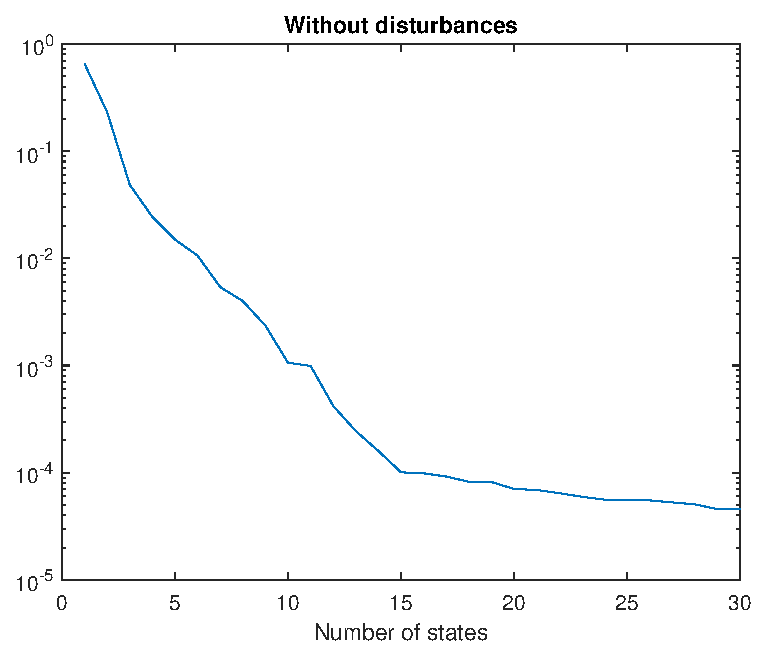
\includegraphics[width=\textwidth]{img/Fig_dump/Sigmas_without_disturbances.eps}
    \caption{$\frac{\Sigma_{i,i}}{sum_{j=1}^{N}(\Sigma_{j,j})}$ from the SVD $U\Sigma V^* = H_1$}
    \label{fig:ERA_state_contributions}
\end{figure}
\todo[inline]{I left off correcting this section @@@. Add the proper figures}
\noindent
From the plot in figure \ref{fig:ERA_state_contributions}, it can be seen that the diagonal elements of $\Sigma$ decrease quite rapidly. Using too many parameters will often cause a mode to be overfitted, which can lead to problems. As a result, models of order 5,7, 10, 12 and 15 were tested. To validate the estimated models, they were plotted against the original step-response. 


\noindent
As can be seen in figure \ref{fig:unscaled_system_approx}, even the 10th order models struggles with estimating certain outputs. This is because the inputs and outputs have not been scaled properly, so the total error will go down significantly more if the error in the $HHV$ is reduced a little, than if the error in $Y_{O2}$ is eliminated. The solution to this is to scale the inputs and outputs somewhat. One formulation for the goal of the scaling can be set is to make as many input-output relations have an amplitude of 1 for some norm (max, $\mathcal{L}_2$, etc.). There is probably a method to finding the optimal solution to this problem, but for the sake of simplicity, it is also possible to alternate between scaling the inputs and the outputs, such that the largest norms, are equal to 1. The exact method is not that important, as long as the HHV or $v_{grate}$ does not dominate the estimation. 

\begin{figure}
    \centering
    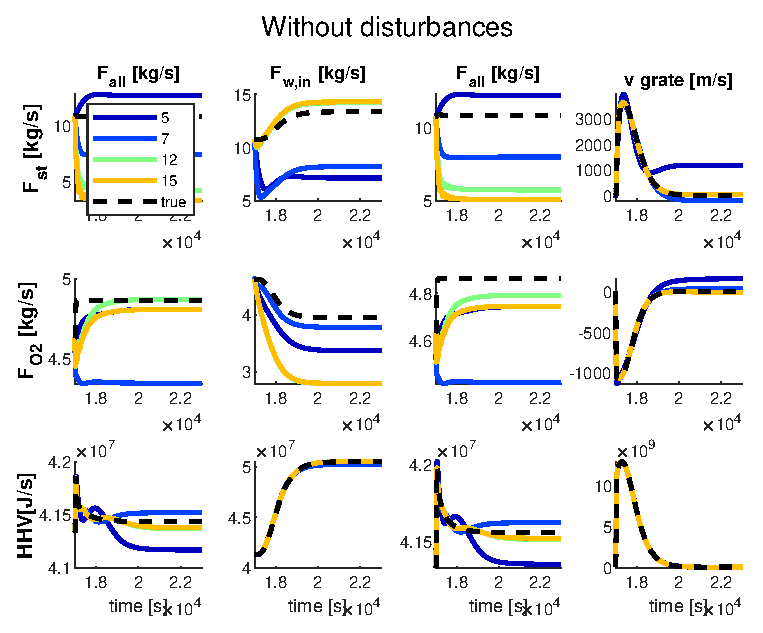
\includegraphics[width=1\textwidth]{img/Fig_dump/Unscaled_ERA_step_approx_without_disturbance_inputs.eps}
    \caption{Approximation from unscaled measurements. The lack of scaling causes an over-fixation on $\hat{HHV}$ and $v_{\text{grate}}$}
    \label{fig:unscaled_system_approx}
\end{figure}



\noindent
After using ERA to estimate the system, it can be scaled back with the same vectors. The result, as seen in figure \ref{fig:proper_system_approx}. The resulting approximated system has a far lower relative error. This scaling is necessary for creating an accurate low-order model that can be used for controlling all outputs of the plant, not just the estimated HHV-value.

\begin{figure}
    \centering
    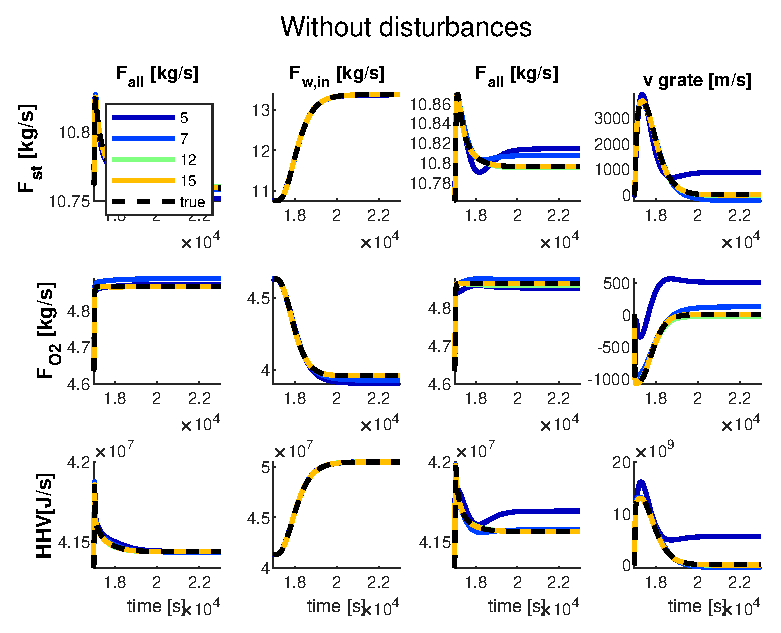
\includegraphics[width=\textwidth]{img/Fig_dump/ERA_step_approx_without_disturbance_inputs.eps}
    \caption{Approximation from scaled measurements. The relative error is now much smaller}
    \label{fig:proper_system_approx}
\end{figure}

\subsection{Choosing a model order}
Picking a model order can be somewhat difficult. From what can be seen in figure \ref{fig:proper_system_approx}. All estimates struggle with matching some of the outputs. Most importantly is the relation between the input air and steam production. Using a model with 7 states might look sufficient at first, but later experiments who that  a model order of 12 was found to greatly outperform it when attempting to control the plant. The reason for why the model has to be so precise is most likely because the controller can get an immediate increase in steam production by increasing $F_{aI}$ while decreasing  $F_{aII}$. If the controller uses this method to suppress immediate changes in steam-production, then this part of the model has to be as precise as possible. 

\subsection{Expanding the model with disturbances}
\todo[inline]{}
Additional experiments were also performed in an attempt to estimate a model for both process disturbances and normal inputs. Figure \ref{fig:ERA_distrubance_state_contributions} shows how much each each state contributes to the new approximation. Figure \ref{fig:ERA_state_contributions} and \ref{fig:ERA_distrubance_state_contributions} are remarkably similar, but the model without disturbances decreases faster in the beginning, which is the reason for why a simpler model can be chosen. 


\begin{figure}%#TODO Add the sigma plot
    \centering
    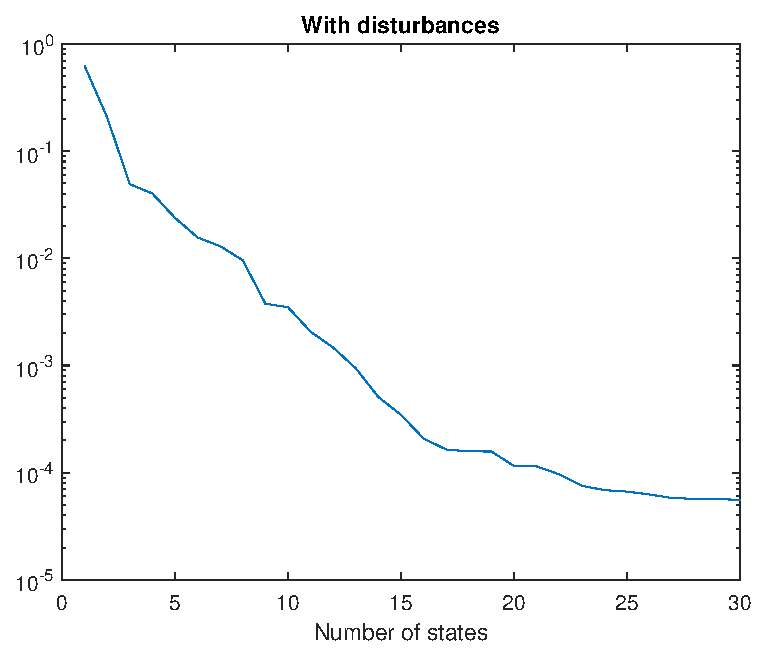
\includegraphics[width=\textwidth]{img/Fig_dump/Sigmas_with_disturbances.eps}
    \caption{$\frac{\Sigma_{i,i}}{sum_{j=1}^{N}(\Sigma_{j,j})}$ from the SVD $U\Sigma V^* = H_1$}
    \label{fig:ERA_distrubance_state_contributions}
\end{figure}



\noindent
Just like in the previous model, the inputs and outputs have to be scaled to get a decent model. Additionally, the extra inputs representing the measurements require a more complex model if everything is to be modelled somewhat properly. As a result, a model of order 15 is used instead of a model of order 12. 

\begin{figure}
    \centering
    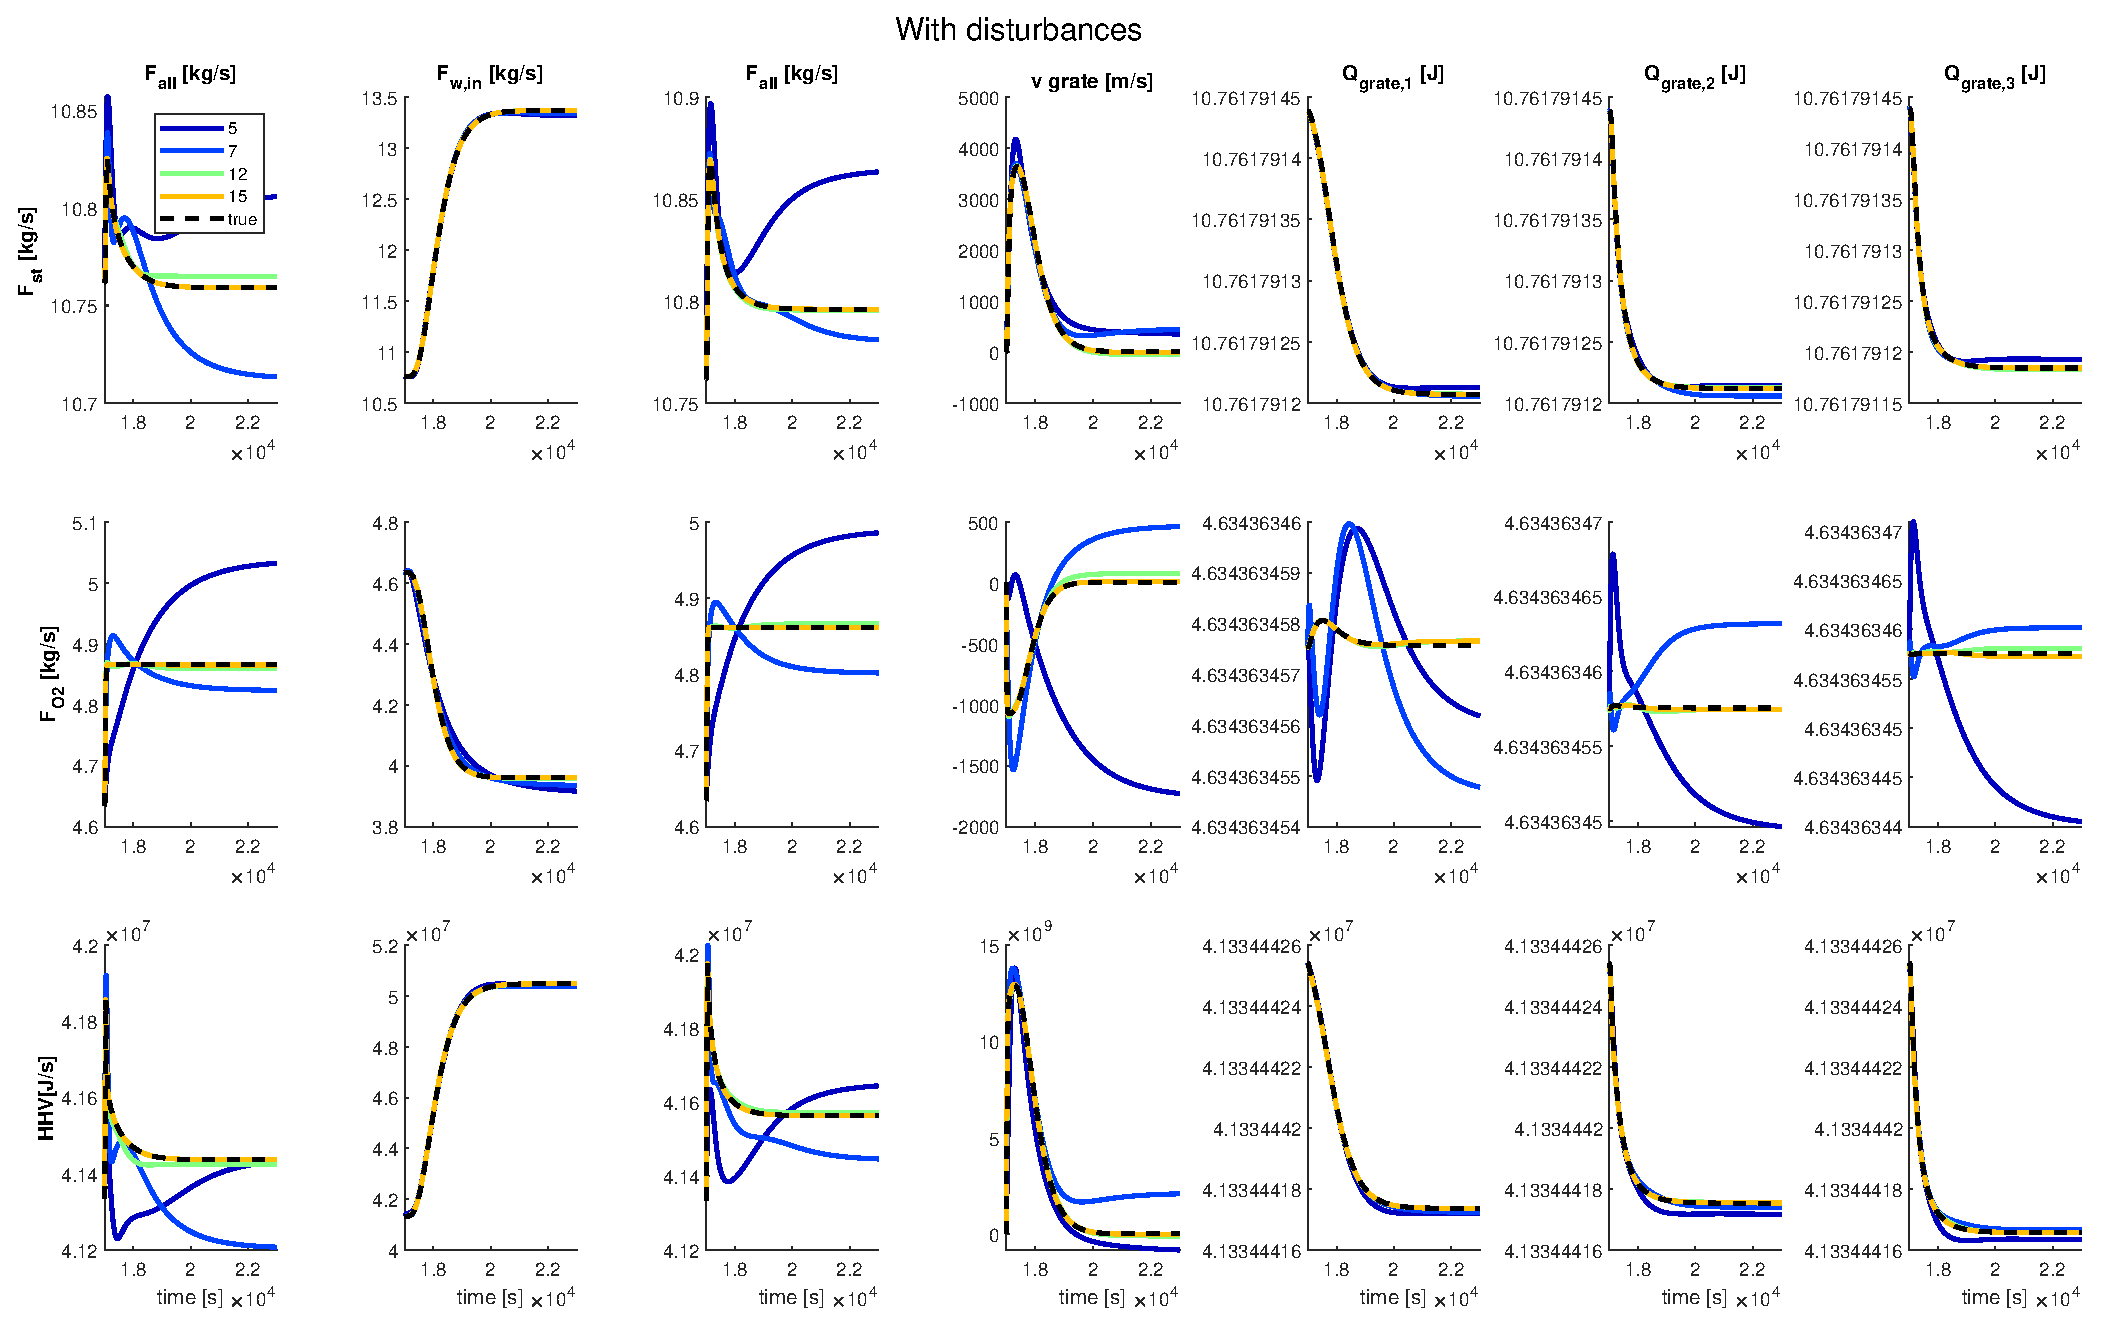
\includegraphics[width=\textwidth]{img/Fig_dump/ERA_step_approx_with_disturbance_inputs.eps}
    \caption{Model that also shows the dynamics of disturbances}
    \label{fig:disturbance_proper_system_approx}
\end{figure}

\noindent 
The estimated response reinforces the notion that Q_grate does not affect $F_{O2}$ very much. This is also the reason as for why the model seems to struggle more with those outputs than most of the other input-output relationships. 


\section{PID-results}

From an earlier project done by a summer-student at SINTEF, another controller has already been implemented. As a result, implementing SIMC or similar tuning methods is almost only interesting from the perspective of showing that it can be done. An easier approach is to make an automatic tuning algorithm that tries to improve on the parameters that have already been used.

\todo[inline]{Add the correct figures here and rewrite accordingly}
\noindent
If the simulator does not take too much time for each simulation, it is possible to automate parts of the tuning process and improve the controller by brute force  if some kind of measure of the quality can be found. Normally, a good measure for the quality of a controller will involve looking at overshoot, settling time and potential stationary deviation. In this case, the cost of the controller is instead deviation $e$ of the theoretical noise-free measurement $y_{\text{noise-free}}$ from the reference value.

\begin{align}
    \text{cost} = \left(\sum_{j=1}^m \sum_{i=1}^N \alpha_j \left(e_{T_i,j} \right)^2\right) + \sum_{j=1}^m \beta \max_{T_i} e_{T_i,j} + \sum \gamma_j \cdot |\sum_{i=1}^N e_{T_{i,j}}| \\
    \label{eq:simulation_cost}
\end{align}

Matlab has an implementation of the Nelder Mead algorithm in accordance to how it was described in \cite{Nelder_Mead_source}. This makes it possible to get good controllers by automatically tuning the parameters during the night. 

\noindent
The main drawback is that the algorithm still requires at least around 1000 iterations to find a really good solution. Additionally, the optimization does not take robustness or noise-rejection if it is not made into a part of the cost. 

An example of the progress of an automated tuning process can be seen in figure \ref{fig:optimization_progress}


\begin{figure}[!ht]
    \centering
    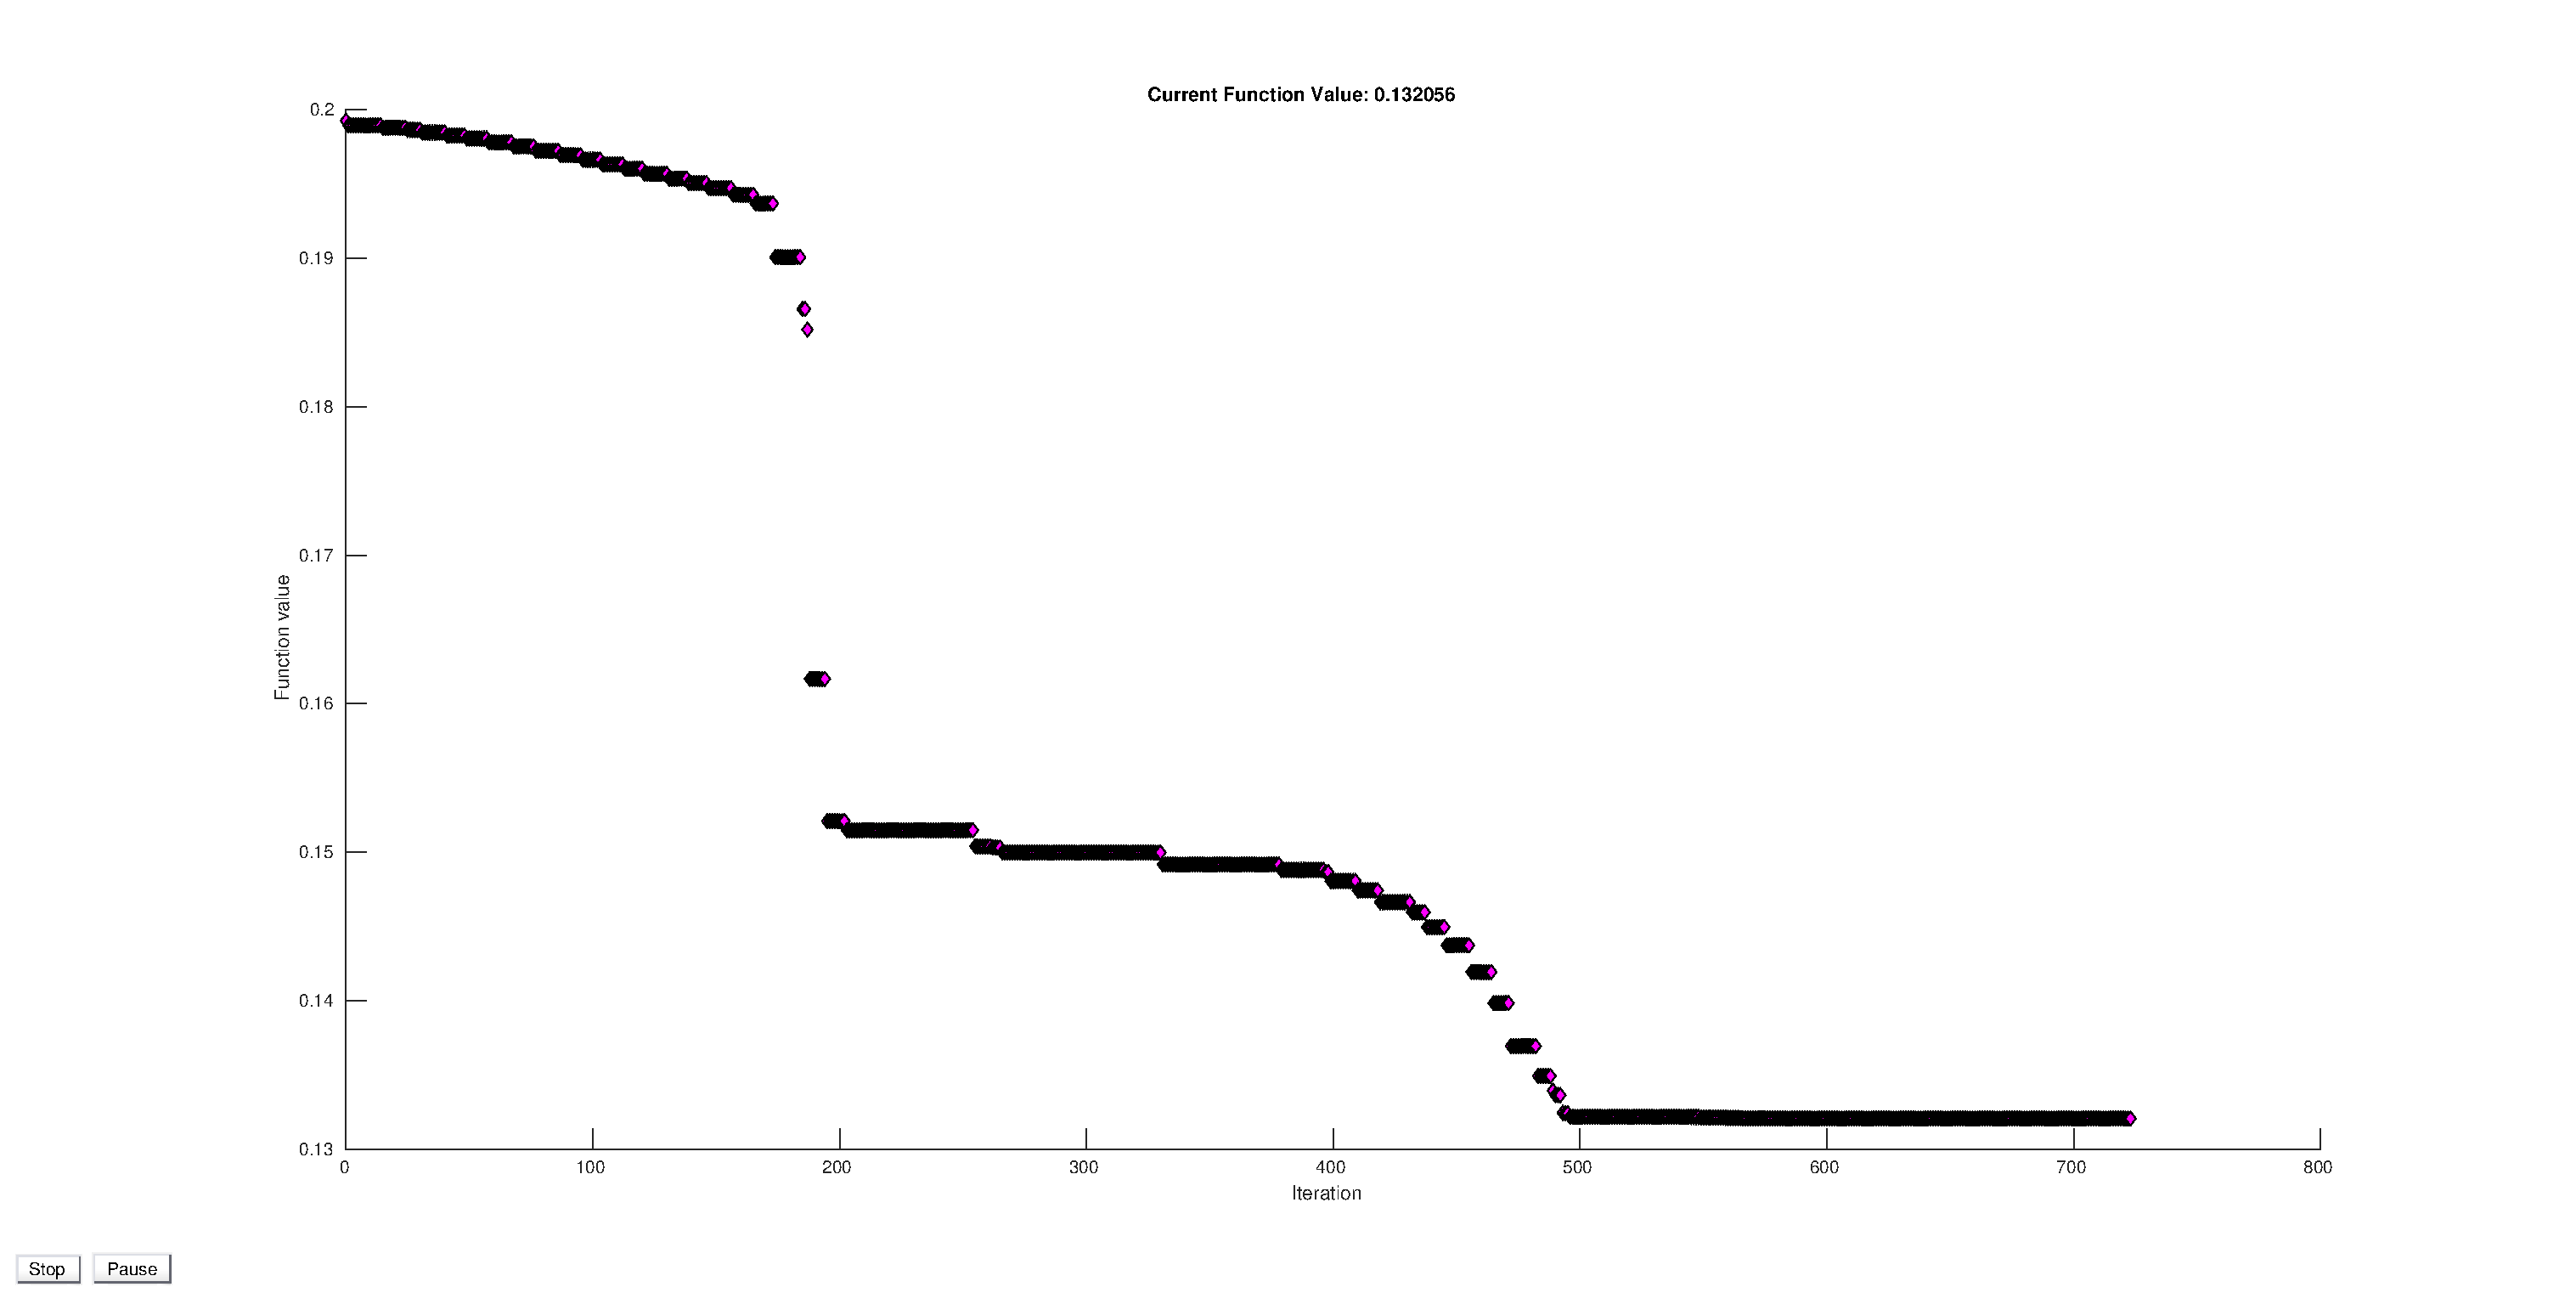
\includegraphics[width=\textwidth]{img/autotune_PID_progress.eps}
    \caption{Norm of $y(t) - y_{ref}(t)$ at each improved time-step of the Nelder-Mead optimization.}
    \label{fig:optimization_progress}
\end{figure}


\subsection{AB-controller}


\begin{figure}[!ht]
    \centering
    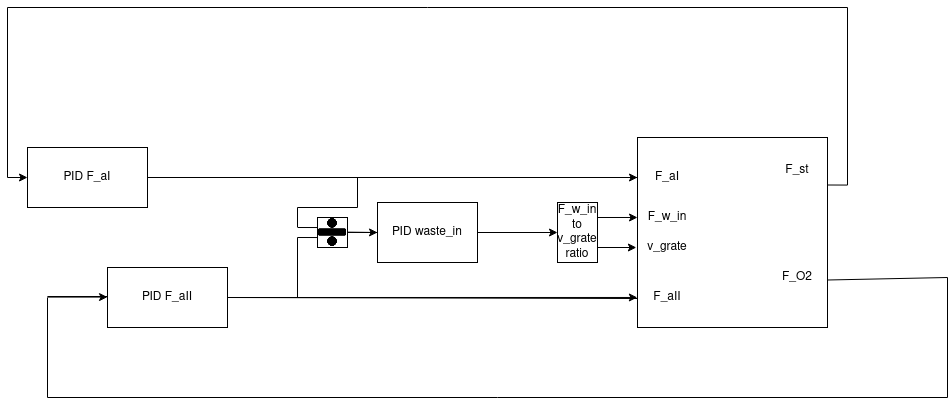
\includegraphics[width=\textwidth]{img/Fig_dump/AB_controller.png}
    \caption{A/B controller structure. Setpoints are assumed }
    \label{fig:AB_controller_structure}
\end{figure}


\noindent
Each output-variable is connected to one input-variable, with the secondary air being used to suppress any changes in the mass-flow of oxygen in the flue gas $F_{O2}$ and the primary air being used to suppress changes in the production of steam $F_{st}$. Using the primary air to control the steam production over long time-horizons is usually a bad idea since both a decent flow of primary and secondary air is needed for the gases to mix properly and for complete combustion to occur. As a result, the ratio between primary and secondary air $\frac{F_{aI}}{F_{aII}}$ is used as the final controlled variable in the plant. The controlled input-variable that is used to make this ratio follow the desired reference is a combination of grate-speed and the mass-flow of waste fed into the combustion chamber. A scaled difference could also have been used, but using a ratio may be desirable. Using too much secondary air is not too bad, beyond the loss of energy that comes from mixing the hot flue gas with ambient air. But using too little is potentially very bad since it might mean producing noxious gases.

\noindent


\begin{figure}[!ht]
    \centering
    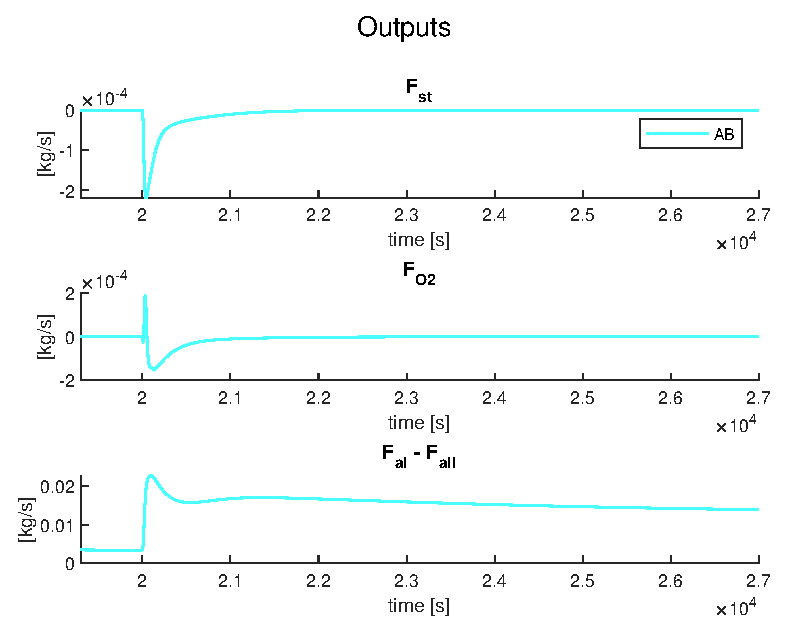
\includegraphics[width=\textwidth]{img/Fig_dump/outputs_ABStep_Q_all.eps}
    \caption{A/B controller disturbance step response}
    \label{fig:AB_outputs}
\end{figure}
\todo[inline]{@@@ Revert these figures to only use AB, instead of AB-cascade}

\begin{figure}[!ht]
    \centering
    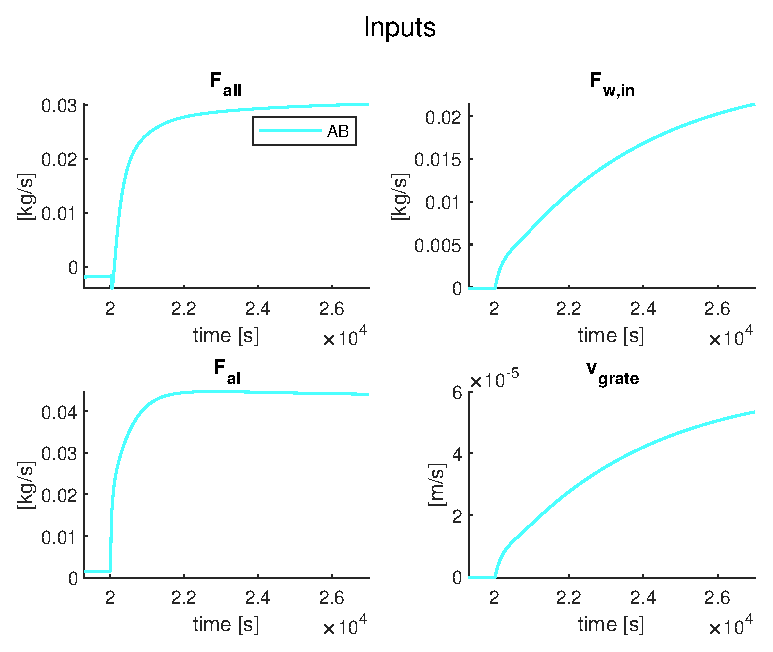
\includegraphics[width=\textwidth]{img/Fig_dump/inputs_ABStep_Q_all.eps}
    \caption{A/B controller disturbance step response}
    \label{fig:AB_inputs}
\end{figure}

Given a sudden step in process-disturbances, the change can be seen in \ref{fig:AB_outputs}. The change involves all three values for $Q_{\text{grate}}$ increasing by 50\%.  Regardless of the amount of measurement.-noise affecting the controller, low-pass filtering the signals still desirable as a safety-precaution. Due to the nature of the simulator having some pure feed-through terms, it is also necessary for completing a simulation. A basic continuous, linear, time-invariant low-pass filter with a time-constant of 0.1 was chosen.

\begin{align}
    \tau_{\text{low-pass}}= 0.1
\end{align}
The noise-spectrum may be very different, depending on the type of method that is used for measuring each variable. A common for of measurement-noise is the hum from the 50Hz AC-grid. The low-pass filter does serve the rejecting the noise from the AC-noise, but if the noise has a frequency-component around 1Hz that is too large, then the result will be far less pretty.

\begin{align}
    |\frac{1}{\left( 50 \cdot 2\pi \right) 0.1j+1}| \approx 0.0318
\end{align}

The response to a 50Hz noise-signal without any system disturbances is show in figure \ref{fig:AB_noise_response}


\begin{figure}[!ht]
    \centering
    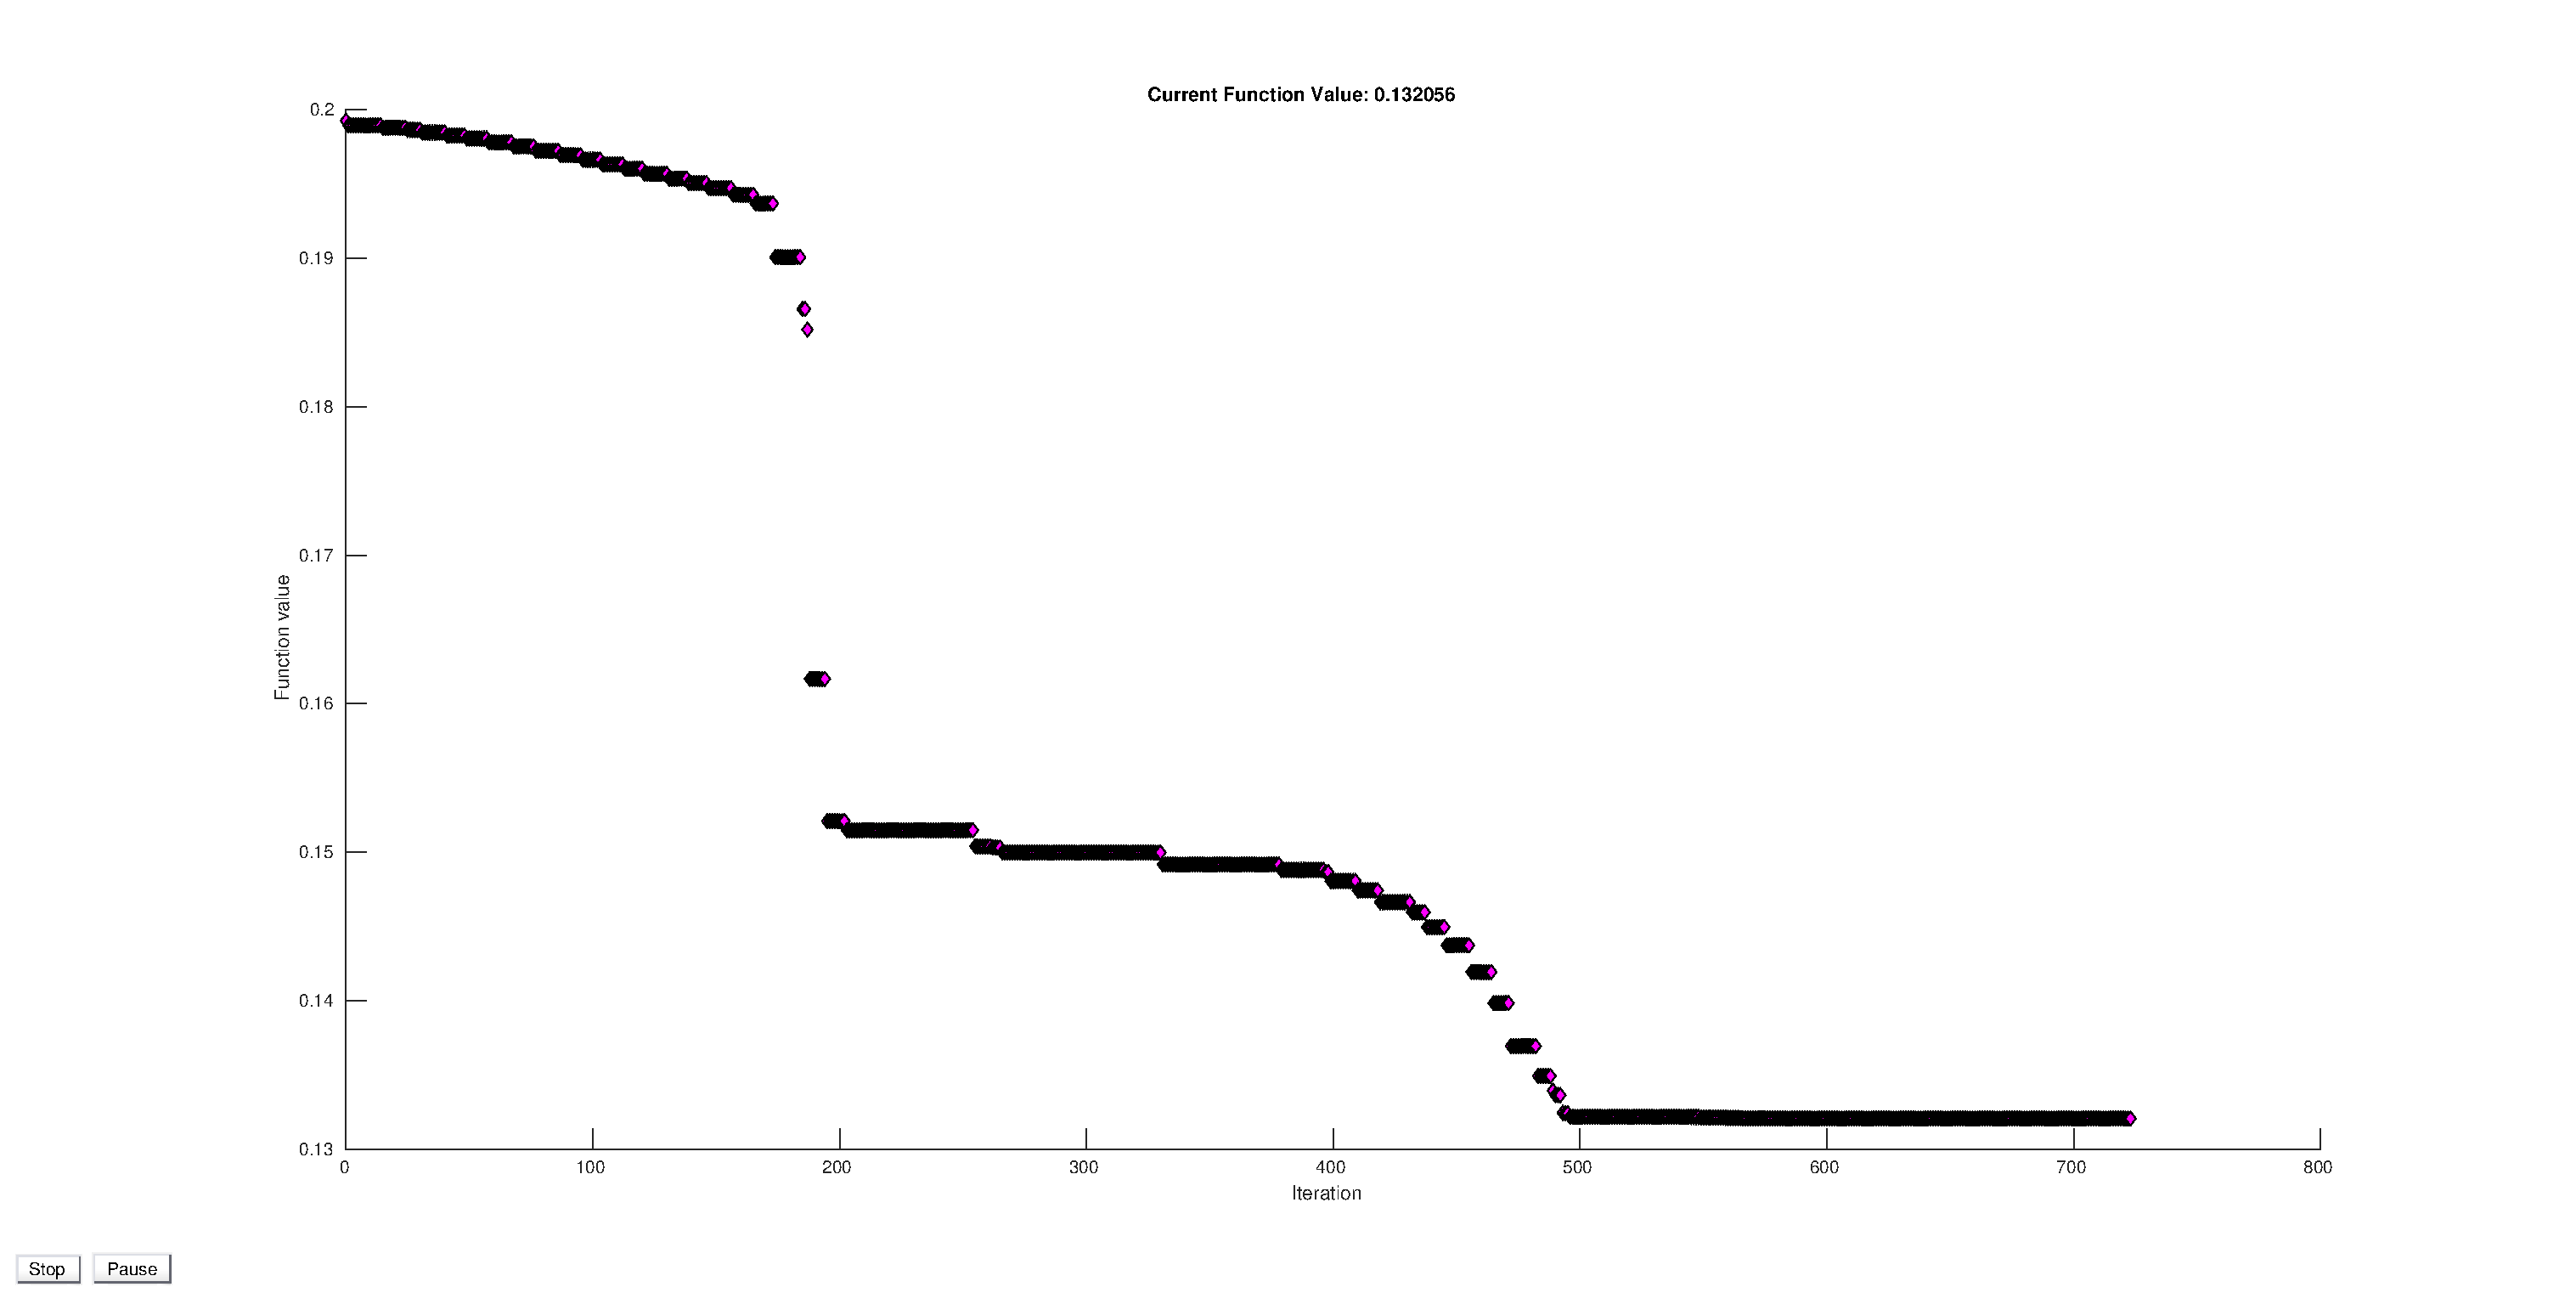
\includegraphics[width=\textwidth]{img/autotune_PID_progress.eps}
    \caption{A/B system noise-response@@@}
    \label{fig:AB_noise_response}
\end{figure}

The resulting response for the oxygen flow  $F_{O2}$ and the steam flow $F_{st}$ can be seen in figure \ref{fig:AB_outputs}.

\subsection{Cascaded A/B controller}
\cite{summer_student} also went on to investigate the possibilities of using a theoretical sensor measuring the heating value of the waste HHV when controlling the plant. The measure proposed there was an estimate

\begin{align}
    \hat{HHV} = \sum_j Cp_j F_{fg,j} \left( T_{fg} - T_{amb} \right)
\end{align}
which is the power delivered to the by a flow of flue-gas. The controller structure, as seen in figure \ref{fig:cascade_controller_structure} is the same as in \ref{fig:AB_controller_structure}, with the exception that the primary air is used to control $\hat{HHV}$, while the controller that tries to control the steam-production gives instead a reflue $\hat{HHV}$. The main advantage of using this controller should be that it can detect changes in the power delivered form combustion earlier, which allows for better control of the steam production. 

\begin{figure}[!ht]
    \centering
    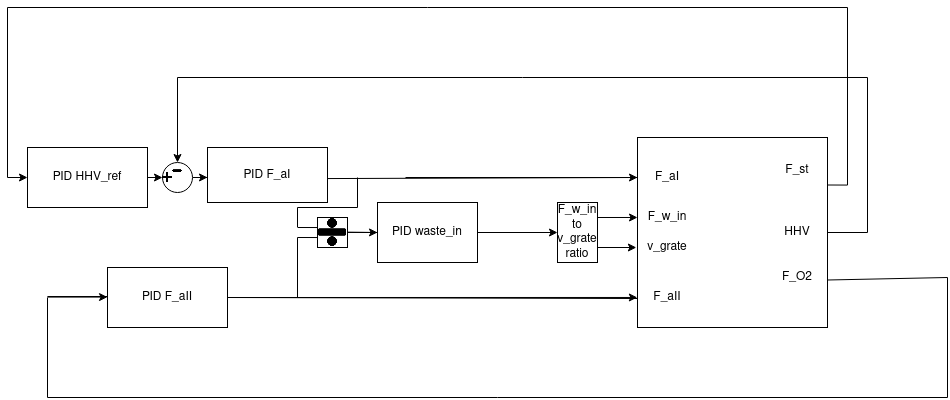
\includegraphics[width=\textwidth]{img/Fig_dump/cascaded_controller.png}
    \caption{Cascaded A/B controller structure}
    \label{fig:cascade_controller_structure}
\end{figure}


As can be seen, from figure \ref{fig:cascade_controller_structure}, both controllers have a rather similar response to changes in the waste quality when it comes to the oxygen concentration. The main advantage of using an estimate of the HHV-value when controlling the plant is the fact that the HHV-value changes before the steam-production, so the cascade controller can suppress the negative peak in the production of steam that happens for both the A/B-controller and the cascaded A/B-controller.

\begin{figure}[!ht]
    \centering
    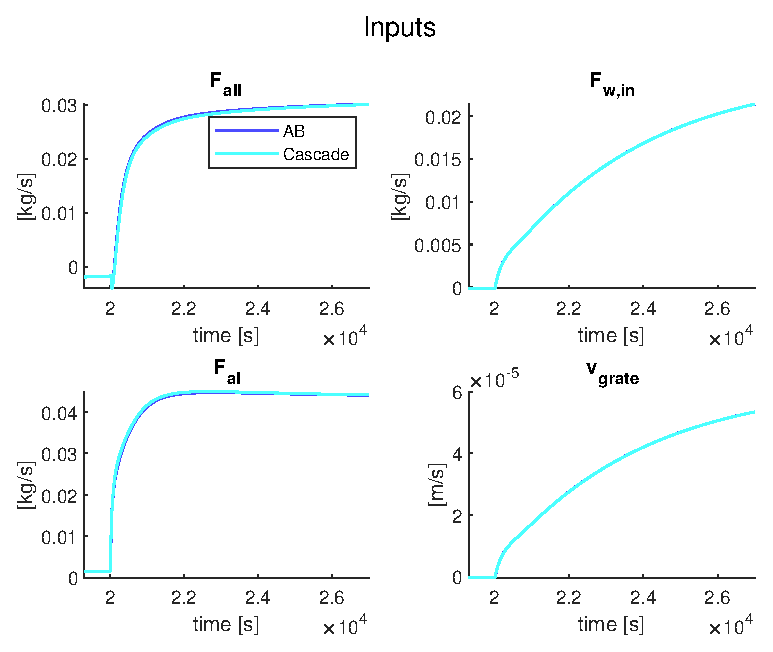
\includegraphics[width=\textwidth]{img/Fig_dump/inputs_ABCascadeStep_Q_all.eps}
    \caption{Cascaded A/B controller disturbance step response}
    \label{fig:cascade_controller_input_response}
\end{figure}




\begin{figure}[!ht]
    \centering
    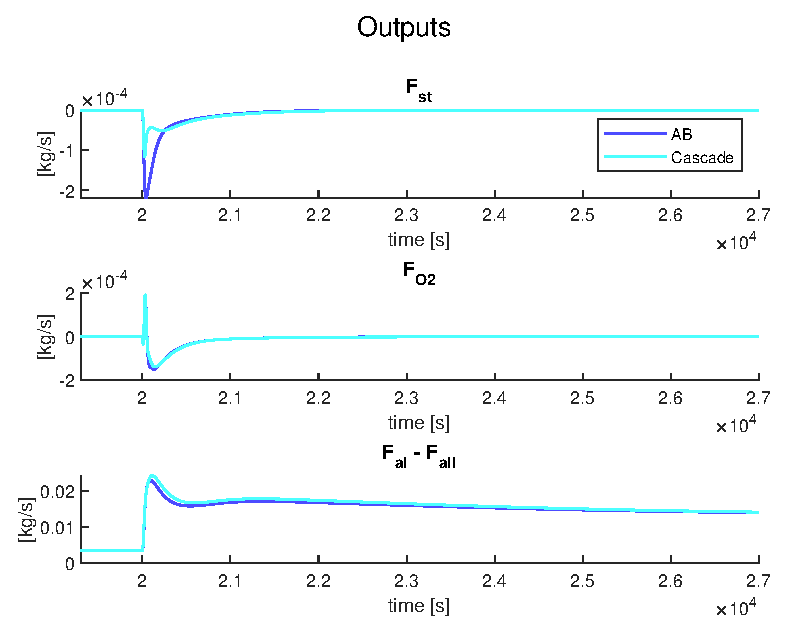
\includegraphics[width=\textwidth]{img/Fig_dump/outputs_ABCascadeStep_Q_all.eps}
    \caption{Cascaded A/B controller disturbance step response @@@ (Remove redundant AB) }
    \label{fig:cascade_controller_output_response}
\end{figure}


Figure \ref{fig:cascade_controller_output_response} has a noticeable in its response. It does not change the total amount of time needed to make the $F_{st}$ converge back to its reference, but the maximum amplitude of the error has decreased significantly. Additionally when looking at the changes in inputs needed to achieve this, figure \ref{fig:cascade_controller_input_response} shows that the inputs are almost identical, with the only difference being very slight differences in timing, with the cascaded controller being marginally more aggressive in its usage of primary air. 




\section{MPC results}
\label{sec:MPC_results}
MPC offers a structure for designing a controller that should be able to stabilize the plant. Nevertheless, there is a multitude of different architectures which may provide different properties. In combination with this, some weights have to be tuned for the controller to prioritize the objectives we want to follow. 

\noindent
Multiple criteria should be upheld.
\begin{itemize}
    \item $F_{st}$ and $F_{O_2}$ should be stabilized and should reject disturbances.
    \item Non-zero mean disturbances should be rejected completely.
    \item The controller should be verifiable through the use of a simulator. 
    \item The ratio between $F_{aI}$ and $F_{aII}$ should only be able to deviate form the pre-determined reference ratio temporarily
    \item In the case where there are hard safety-constraints, the controller should try to uphold these. 
    \item The controller should be well-behaved, even if the inputs have saturation limits or limits to the rate of change. 
\end{itemize}

\noindent 
Normally, an MPC differs somewhat from an LQR in that it can express a cost for the change in variables. The LQR usually has to use high-pass filters to achieve a similar effect. Fortunately, a low-pass filter on the input is already required to control the plant, since both MPCs and simulators are bad at handling feed-through terms through the plant and controller. As a result, the low-pass filter can be used to make a high-pass filter:

\begin{align}
   1 - \frac{1}{\tau_{\text{low pass}} s +1} = \frac{\tau_{\text{low pass}}s}{\tau_{\text{low pass}}s +1} = h_{\text{high pass}}(s)
\end{align}

\noindent
Matlab already has a function $\text{lqry}$, which returns the gain $K_{lqr}$. $K_{lqr}$  optimizes the Ricatti equation if an output-cost $Q_y$ and a state-cost $R$ is provided. An optional cost matrix, $N$, which punishes or rewards certain combinations of $x$ and $u$ is also used to implement the punishment for changing the inputs too much.

\begin{align}
    K_{lqr} = \text{lqry} \left( \text{lqry_plant}, Q_y, R, N \right)
\end{align}
$\text{lqry}$ should be used instead of normal $\text{lqr}$, since performing the multiplication $Q = C^T Q_y C$ may break the positive semi-definiteness of $Q$, due to numerical errors. Any cost that may instead result from changes in input or output can be expressed by expanding the observed states


\begin{align}
    C_{lqr} = \begin{bmatrix}
        C\\
        C_{\text{input_filter}}\\
        C\left( A - I \right)
    \end{bmatrix}
\end{align}




\noindent
Nelder-Mead can be used to optimize the costs in the controller and estimator. Because MPCs and LQR are usually tuned by multiplying the weights of factors 10, it is paramount that the optimized vectors represent exponents of 10, as the alternative would lead to very poor convergence. As for now, it is assumed that all forms of noise and disturbances are uncorrelated, so both $R_{lqe}$ and $Q_{lqe}$ are made to be diagonal matrices. The same is done for $Q_y$ and $R$, which is used by the controller. Tuning the plant completely blindly can often be a bad idea since it can lead to several unneeded steps before reaching any decent results. There is no guarantee that the problem is truly convex, so it might be preferable to tune the controller manually until it does a decent job. 
\todo[inline]{Add an initial guess here}

\subsection{Different LQE structures}
Section \ref{sec:ERA_results} showed two different kinds of models, one where the disturbances were measured, and one where they are almost ignored completely. An LQE usually needs some measure of variance with regards to measurement noise and process disturbances. By using data that is somewhat representative of process-data, it should, in theory, be possible to create a good LQE only by using the estimated model and those measures. In practice, the resulting controllers struggled significantly and performed worse than the PID-controllers, as shown in figure \ref{fig:Assuming_controllers_outputs}. 

\begin{figure}
    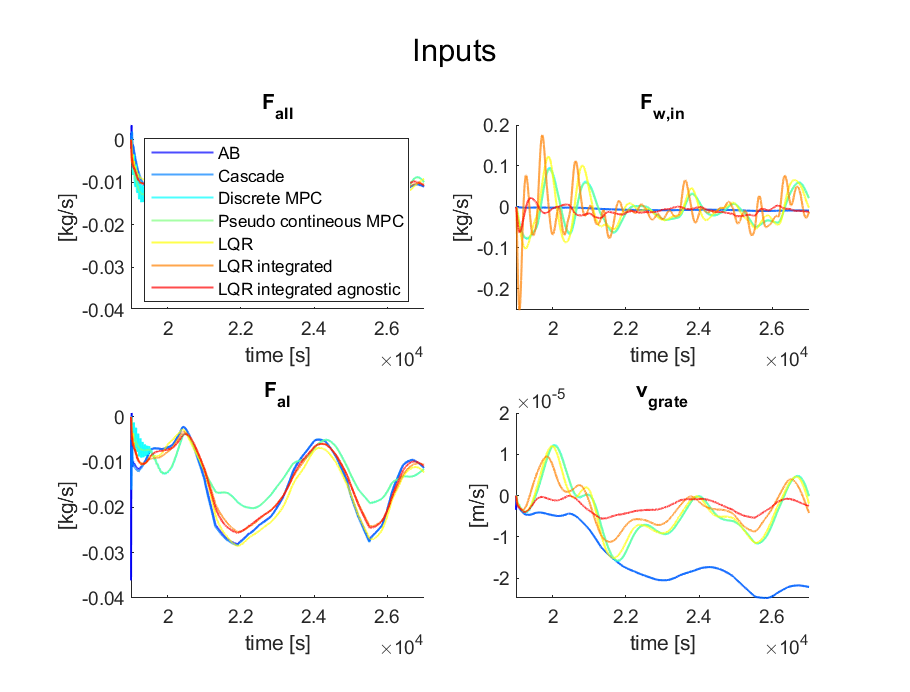
\includegraphics[width=\textwidth]{img/Fig_dump/outputs_ABCascadeDiscrete_MPCPseudo_contineous_MPCLQRLQR_integratedLQR_integrated_agnostic.eps}
    \label{fig:Assuming_controllers_outputs}
    \caption{Comparison of the different controllers with stochastic disturbances}
\end{figure}
\todo[inline]{@@@ Remove the stochastic plot}
\noindent
The solution to this would normally be a rather unpleasant one, as it involves tuning the expected disturbance for each state, and the expected noise for each input. Luckily, it is not so hard to make an estimator that functions decently, and that can stabilize the plant in combination with a gentle controller. As a result, tuning the estimator becomes part of the optimization tuning problem. 
\todo[inline]{Say something about estimators with measurements}

\subsection{Integral LQR}
Almost any model predictive controller that is not overly aggressive should be able to fulfil point 1. The second one is a bit more tricky, but the normal solution to this is to add integral states to all controlled outputs. This also has the added benefit of allowing reference tracking, even without explicitly creating a feed-forward matrix. The easiest way to get integral action for the outputs is to expand the state-space

\begin{align}
 A_{I} =& 
 \begin{bmatrix}
 A & 0 \\
 I & 0
 \end{bmatrix}\\
 B_{I} =& 
 \begin{bmatrix}
 B \\
 0
 \end{bmatrix}\\
 C_{I} =& 
 \begin{bmatrix}
 C & 0 \\
 0 & I
 \end{bmatrix}\\
  D_{I} =& 
 \begin{bmatrix}
 D \\
 0 
 \end{bmatrix}\\
\end{align}

\begin{figure}
    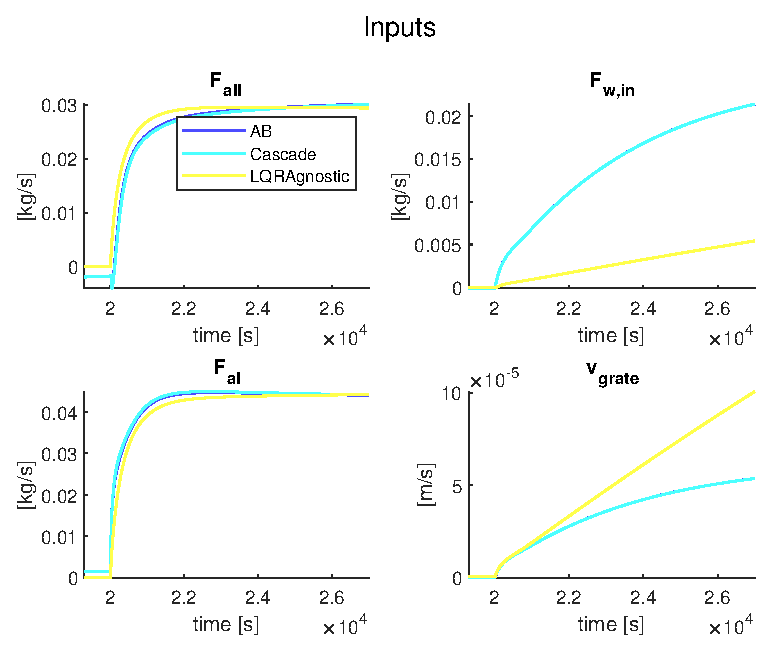
\includegraphics[width=\textwidth]{img/Fig_dump/inputs_ABCascadeLQRAgnosticStep_Q_all.eps}
    \label{fig:integral_controller_comparison}
    \caption{Normal integral cost LQR vs PID}
\end{figure}

\begin{figure}
    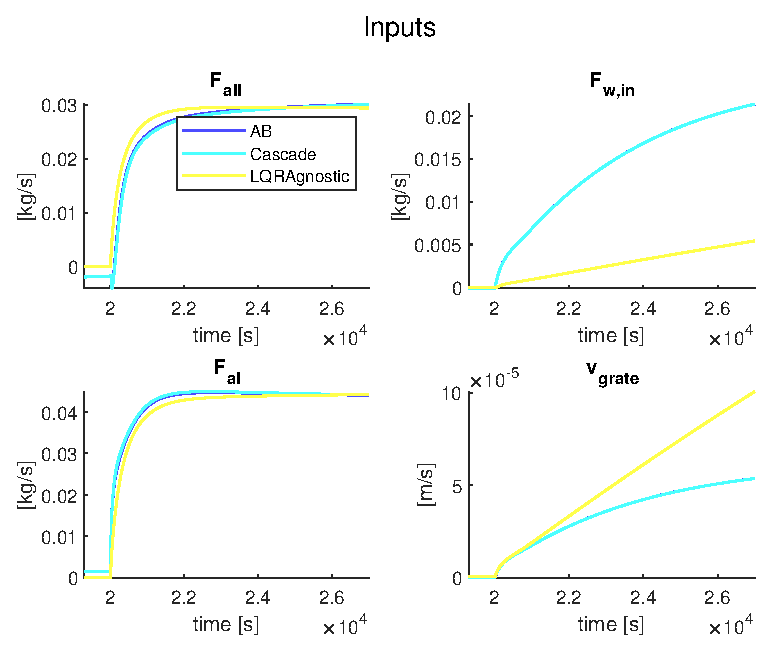
\includegraphics[width=\textwidth]{img/Fig_dump/inputs_ABCascadeLQRAgnosticStep_Q_all.eps}
    \label{fig:integral_controller_comparison_inputs}
    \caption{Normal integral cost LQR vs PID}
\end{figure}
\todo[inline]{Change the figures to how they reject noise instead}

\noindent
As can be seen in figure \ref{fig:integral_controller_comparison}, the linear quadratic controller still loses to the PID-controllers on some points. Mostly in regards to steam production and $O_2$ concentration. The reason for this is most likely some 
\todo[inline]{Should I say that it probably stems from a modeling error}

. The main draw-back is that the LQR-controller has an unintended change in the amount of air released. This also happens to the PID, but that is because the selected ratio between primary and secondary air is chosen to be different from 1.  Even if aggressive usage of primary and secondary air can be a useful tool for handling disturbances, changes in grate-speed and waste-flow should be the preferred method for handling persistent changes in waste-composition. It is possible to give an additional cost for whenever $F_{aI}$ and $F_{aII}$. The resulting controller, as seen in figure \ref{fig:integral_controller_with_air_diff_cost} loses a lot of its ability to reject disturbances properly, while also being somewhat robust.


\begin{figure}
    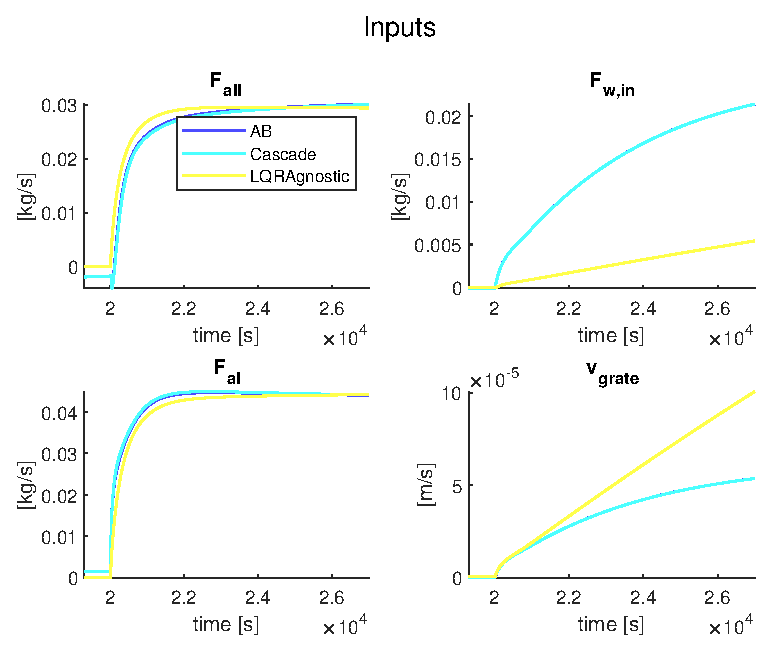
\includegraphics[width=\textwidth]{img/Fig_dump/inputs_ABCascadeLQRAgnosticStep_Q_all.eps}
    \label{fig:integral_controller_with_air_diff_cost}
    \caption{LQR versus PIDs}
\end{figure}

\begin{figure}
    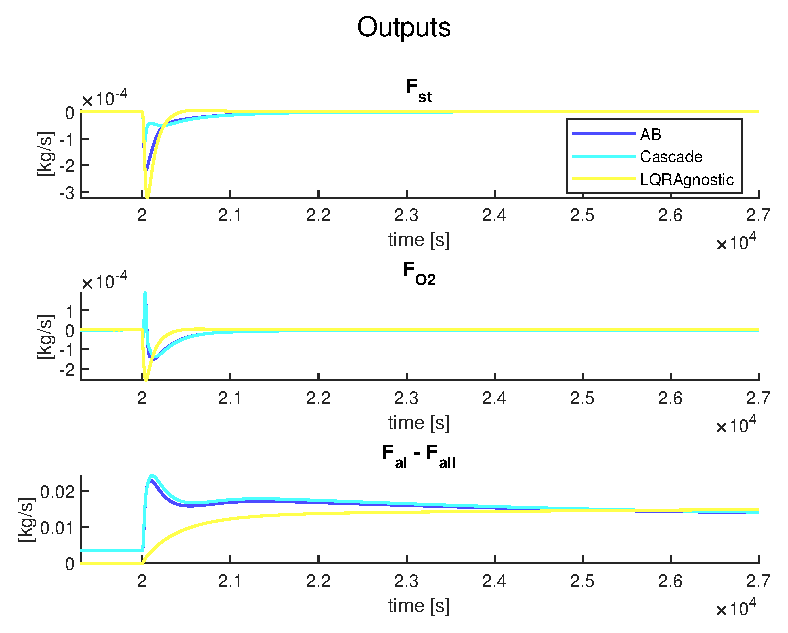
\includegraphics[width=\textwidth]{img/Fig_dump/outputs_ABCascadeLQRAgnosticStep_Q_all.eps}
    \label{fig:integral_controller_with_air_diff_cost_inputs}
    \caption{LQR versus PIDs}
\end{figure}

\todo[inline]{Say something about the differences if it can not be fixed}
\subsection{LQR with integral cost on \texorpdfstring{$F_{aI}-F_{aII}$}{TEXT}}
Balancing the normal costs, trying to reject disturbances, while also enforcing a decent ratio between $F_{aI}$ and $F_{aII}$ may prove to be a pointless endeavour. It may also mean not using a very useful tool for rejecting disturbances since allowing the two air-flows to temporarily deviate has a faster response than changing the amount of waste ted into the furnace. The intuitive solution to this is to add an integral cost to  $F_{aI}-F_{aII}$ instead, and then giving it a rather low priority compared to the other objectives. The resulting response is shown in figure \ref{fig:integrall_diff_cost_outputs}

\begin{figure}
    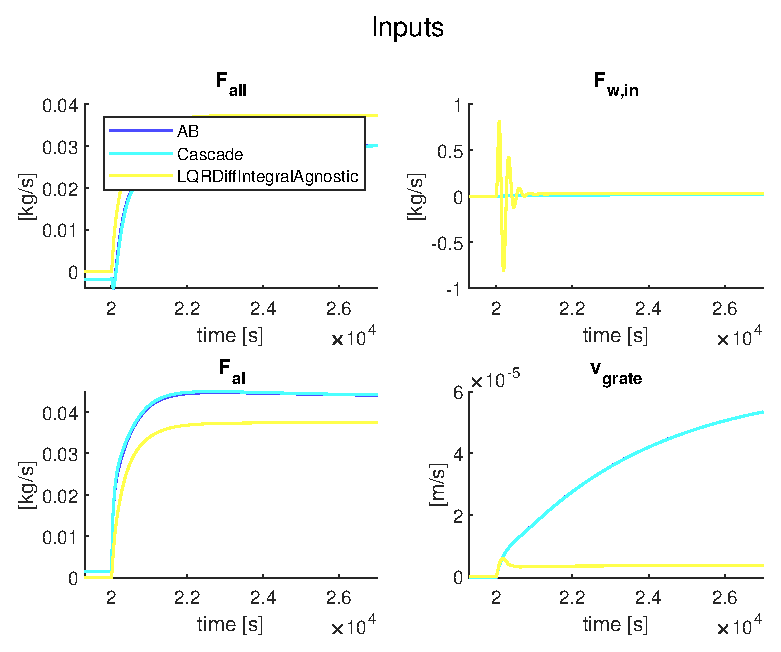
\includegraphics[width=\textwidth]{img/Fig_dump/outputs_ABCascadeLQRDiffIntegralAgnosticStep_Q_all.eps}
    \label{fig:integrall_diff_cost_outputs}
    \caption{PID vs LQR with intefral cost on $F_{aI} - F_{aII}$}
\end{figure}

\begin{figure}
    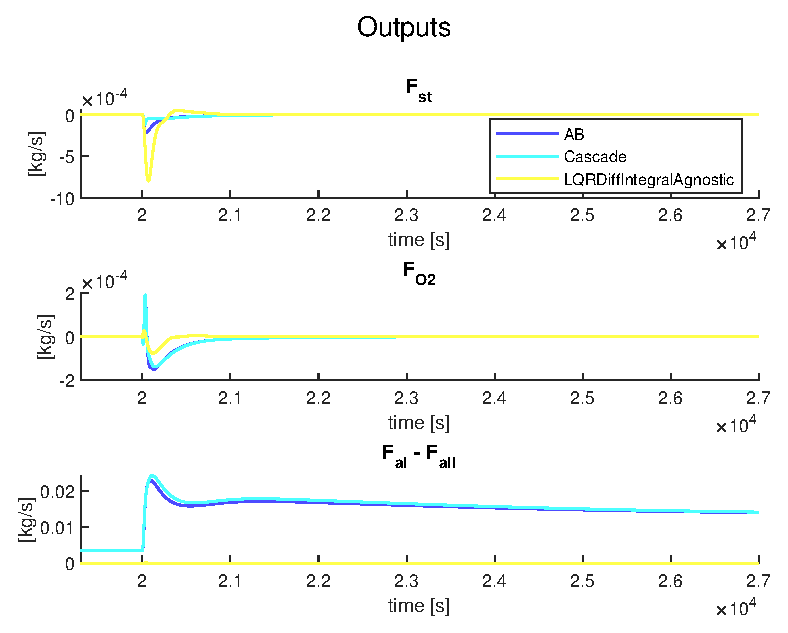
\includegraphics[width=\textwidth]{img/Fig_dump/inputs_ABCascadeLQRDiffIntegralAgnosticStep_Q_all.eps}
    \label{fig:integrall_diff_cost_inputs}
    \caption{PID vs LQR with intefral cost on $F_{aI} - F_{aII}$}
\end{figure}


\todo[inline]{C@@@ omment the results (The current ones are form an over-sensitive controller, so it might be bad...)}
% \subsection{}

\subsection{Discrete MPC}

\todo[inline]{@@@ Add an actual plot of a discrete MPC}
Even if a rather low sampling-time might work well for an MPC in practice, it does not work as well with the simulator, due to the stiffness of the problem. As a result, a sampling-time of 20 had to be chosen, even though that is noticeably slower than the preferable sampling-time of somewhere around one second. As a result, the MPC will have objectively worse performance than the LQR as long as all inequality-constraints are inactive. The delay means that the weight used for the LQR may not work as well for an MPC. The simulation will also run more slowly when an MPC is involved.
\begin{figure}
    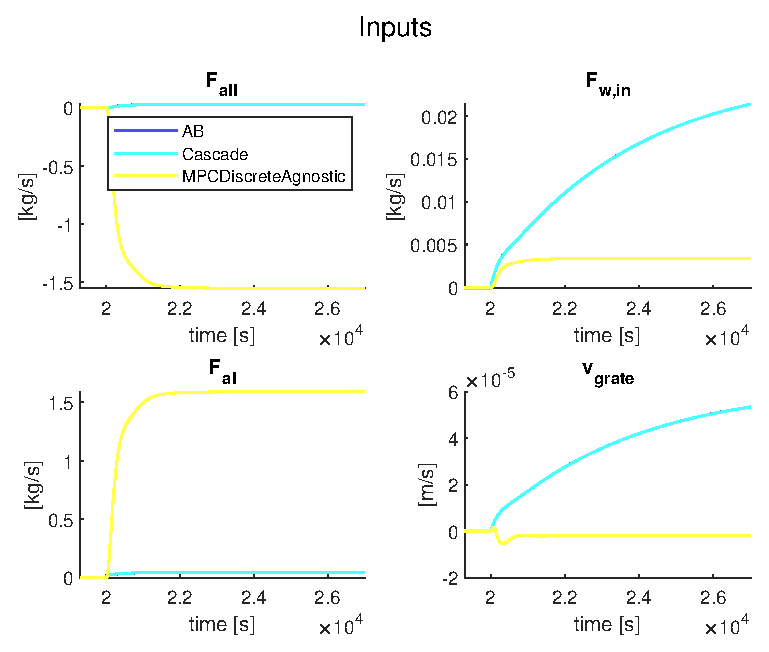
\includegraphics[width=\textwidth]{img/Fig_dump/outputs_ABCascadeMPCDiscreteAgnosticStep_Q_all.eps}
    \label{fig:discrete_mpc_outputs}
    \caption{Comparison of the different controllers with stochastic disturbances@@@}
\end{figure}

\begin{figure}
    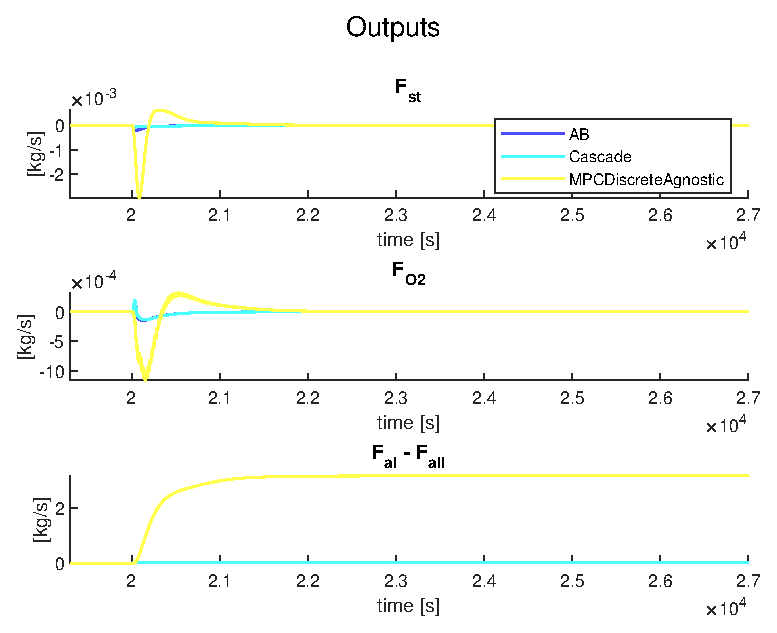
\includegraphics[width=\textwidth]{img/Fig_dump/inputs_ABCascadeMPCDiscreteAgnosticStep_Q_all.eps}
    \caption{Comparison of the different controllers with stochastic disturbances@@@}
\end{figure}



\section{Robustness analysis}

\todo[inline]{This section is not complete@@@}
Even though the system is stable with the model that has been given, the assumptions that were made may be somewhat incorrect. As a result, the constructed controller should preferably also have at least some robustness against modelling errors. This analysis will only focus on errors in input gain and on time-delays. All models described in this section will be of continuous LTI systems. 


\subsection{Combined estimator and physical system}

The physical plant, and the one used by the MPC are not entirely the same. As a result, some extra steps have to be taken when representing both the physical system and the estimated one in the same state-space. This analysis will only go over input-delays and not output-delays. 


\noindent
Let $A$,$B_p$,$C$ and $D$ represent the physical system and the matrix $B$ input matrix of the estimated system. Finally, let $K_{lqe}$ represent the feedback mmatrix used by the linear quadratic estimator.  Then the open-loop system between the real state and the estimated state can be written as:

\begin{align}
    \begin{bmatrix}
        x\\
        \hat{x}
    \end{bmatrix}
    = 
    \begin{bmatrix}
        A & 0 \\
        K_{lqe} C & A - K_{lqe} C
    \end{bmatrix}
    \begin{bmatrix}
        x\\
        \hat{x}
    \end{bmatrix}
    + 
    \begin{bmatrix}
        B_p\\
        B
    \end{bmatrix}
    u
\end{align}

The controlled system is not necessarily the same as the estimated system. A low-pass filter has to be used by the controller or estimator to make remove all feed-through terms from LTI-system. This low-pass filter is represented by the matrices $A_F$ , $B_F$ and $C_F$. Additionally, the controlled states are not necessarily the same as the measured outputs, so a different pair of matrices $C_c$ $D_c$ are used to axtract them form the estimate. Said measurements are used for making the integrator states of the plant. Finally, a padé-approximation is needed for the delay between the input-filter and the rest of the process. The delay will be estimated by $A_D$, $B_D$, $C_D$ and $D_D$. 

The full system is divided into several smaller sub-systems. 
\begin{align}
    x_{full}
    \begin{cases}
        x_{\text{physical}}\\
        x_{\text{estimated}} \\
        x_{\text{input filter}}\\
        x_{\text{integrated outputs}}\\
        x_{\text{padé approxomation}}\\
    \end{cases}
\end{align}

\begin{align}
    A_{full} 
    = 
    \begin{bmatrix}
        A        & 0            & B_p D_D C_{F} & 0   & B_p C_D          \\
        K_{lqe}C & A - K_{lqe}C & B C_F         & 0   & 0           \\
        0        & 0            & 0             & A_F & 0         \\
        C_c      & 0            & D D_D C_F     & 0   & D C_D   \\
        0        & 0            & B_D C_F       & 0   & A_D   \\
    \end{bmatrix}
\end{align}

\begin{align}
    B_{full}   =
    \begin{bmatrix}
        0 \\
        0 \\
        B_F \\
        0 \\
        0
    \end{bmatrix}
\end{align}

Instead of using normal states as outputs, it is also possible to translate them directly into the corresponding optimal set of inputs. The matrix $K_{lqr}$ uses the estimated states, as well as the filtered states and the integrated states. 

\begin{align}
    C_{full} = 
    \begin{bmatrix}
        0 & K_{lqr} & 0
    \end{bmatrix}
\end{align}

Because of the low-pass filter, $D_{full}$ is always 0. The stability of the feedback loop can be analysed by adding a padé approximation of a delay in the feedback between the optimal next input given out by $C_{full}$ and the input used on $B_{full}$. 
\noindent

\subsection{The root locus plots}
With a fully functioning state-space system of both the physical system and the estimated one, it becomes possible to say something about how the poles evolve, depending on delay and static gain error. To test the static gain error, it is simply sufficient to multiply $B_p$ 
by some constant. The robustness to delay can be tested by adding a padé- approximation in the feedback-loop, of some pre-determined order, and then setting the desired delay. In this analysis, order 9 was chosen, although there may be reasons for choosing other padé-approximations as well. 

In this section, the LQR-controller with integral cost on $F_{aI} - F_{aII}$ will be covered, since it was one of the best-performing architectures. 

\begin{figure}
    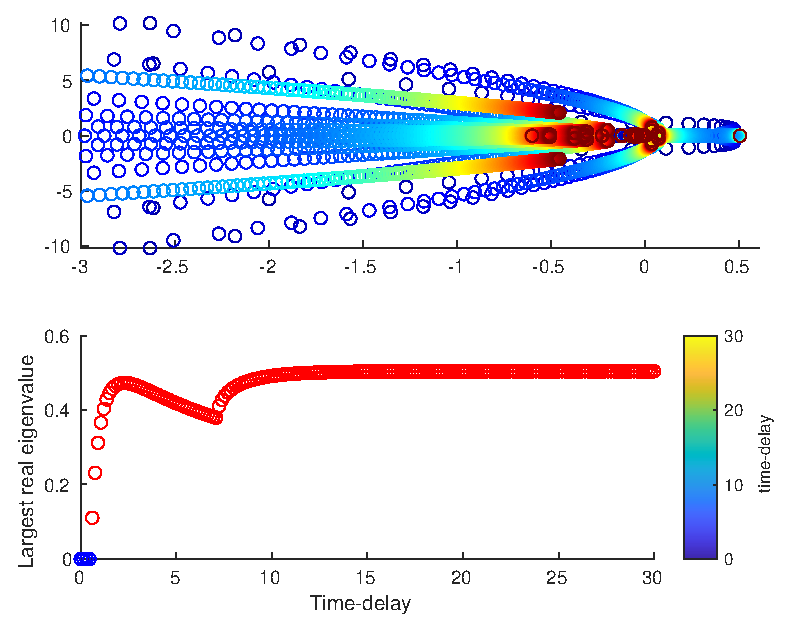
\includegraphics[width=\textwidth]{img/Fig_dump/tau_root_locusLQRDiffIntegralAgnostic_paramsfor_all.eps}
    \label{fig:LQR_root_locus_full_delay}
    \caption{Root locus plot for delays on all plant inputs}
\end{figure}

The controller is quite sensitive to time-delays from the results in figure \ref{fig:LQR_root_locus_full_delay}, becoming unstable if all inputs suffer an input-delay of only 0.3 seconds. If it can be guaranteed that there will be some inputs without delays, some stronger guarantees can be given instead. A delay of 5 seconds can be tolerated if there is no delay in the grate-speed. Sadly, this input that gives a notable improvement is if $v_{grate}$ .


\noindent 
The fact that $v_{grate}$ is one of the most problematic inputs was not something that could be solved in this project. It is especially bad, since it would seem more reasonable that the fans have a lot less variance in their delay compared to the ram and the grates, simply because they are a lot faster. In theory, decreasing the reliance on $v_{grate}$ should make it better, but no solution was found during this project that also resulted in performance that could rival the previous controller. There may be some solution, using a different architecture or bu using a different set of weights. 



\begin{figure}
    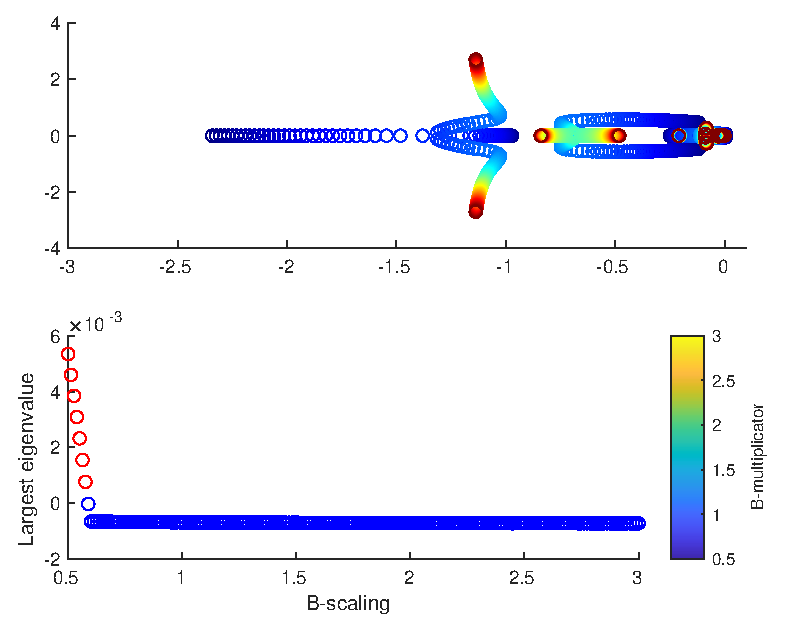
\includegraphics[width=\textwidth]{img/Fig_dump/B_scaling_root_locusLQRDiffIntegralAgnostic_params.eps}
    \label{fig:LQR_root_locus_B}
    \caption{Root locus plot for linear scalings of B}
\end{figure}



\todo[inline]{Check if this is complete @@@}
\begin{figure}
    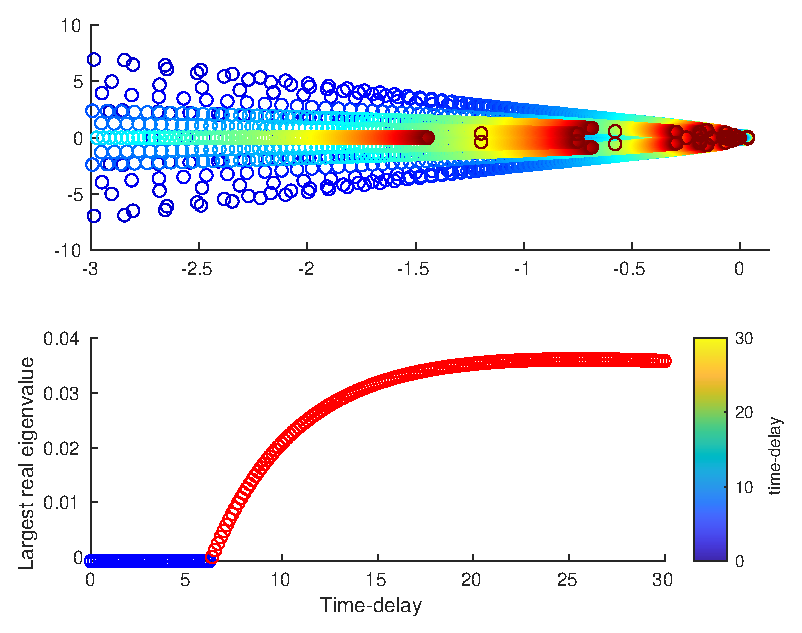
\includegraphics[width=\textwidth]{img/Fig_dump/tau_root_locusLQRDiffIntegralAgnostic_paramsair_diff.eps}
    \label{fig:LQR_root_locus_air_safe}
    \caption{Root locus plot for unmodeled time-delays}
\end{figure}



%!TEX root = ../Thesis.tex
\chapter{Conclusions and future work}\label{cha:conclusions}

\todo[inline]{
This is a summary of the results of the report, and here you also describe future work (For the preliminary project: what you are going to do in your MSc project work, and for the master´s project: what you would do if you had 6 more months to work on this topic.)
}
\section{Conclustion}
\todo[inline]{@@@ This is the most important part to add @@@}

The task of controlling an MSW combustion process proved to be a difficult one. This project provided the luxury of working with a simulator, which gave a rich source of potential data, as well as possibilities to verify the results. This also proved to be at the core of the issue, since certain kinds of controllers could not be implemented, due to the simulation time going towards infinity, or the simulator crashing with unknown errors, if the controller had discrete samples that were too frequent. 

\noindent
In the project, the ERA  was implemented, allowing for estimating the dynamics of a linear system with unmeasured internal states was implemented. Furthermore, several different LQR and MPC controllers were implemented. Hard limits on the input-variables were also added to the MPC to better allow it to handle saturation, but this never became relevant with the disturbance test-data that was available. Hard limits on the measured outputs, with slack variables  were also implemented, but the results were never discussed properly, due to them never being enforced. Due to what is assumed to be minor errors in implementation, the LQR-controller was not able to outperform the PID-controllers. There were, however several more positive outcomes. A root-locus method was implemented for estimating the stability of a closed-loop estimated system. Additionally, a simple method for automatically tuning the PID- controller and the optimal controllers was also implemented. 

\noindent 



\section{Future work}
The purpose of this project was to develop a controller that could outperform the current PID-controller. This was only achieved in part since the current PID-controller was improved by the process of automated tuning. 
There are a multitude of different things that could be done if more time is was available. 
\begin{itemize}
    \item The most important improvement is the fact that there was most likely something wrong in how the estimated plant was made into an observed plant, a controlled plant, and how these states were used afterwards. 
    \item Implement some estimate for the robustness of the current PID-controller. Most likely by using the ERA to make open-loop models that can be analyzed. 
    \item Feed-forward control on the plant was implemented, but had some strange behaviour, even in the most ideal of cases. Further exploration of that could have been useful, but even the most idealized cases were somewhat limited in what they could achieve. 
    \item Using integrators instead of low-pass filters could, in theory, implement a better way to limit the controller from changing the inputs too quickly. 
\end{itemize}

\section{Conditionally useful improvements}
Some of the potential future work are relatively large tasks, and should not be pursued unless there are explicit observations that prove them to be needed. 
\begin{itemize}
    \item If the true test-data make the nonlinearities in the plant more prominent, a simplified nonlinear model could be implemented with nonlinear methods like simple linear regression, or the more advanced SINDy-algorithm. But these methods usually require full-state measurement. 
    \item Proper analysis of process-disturbances and measurement-noise should be implemented since it might show the need for specialized band-stop filters. 
    \item Exploration of how the performance degrades if the estimated HHV-value is not available. 
    \item An exploration of what measurement-techniques are available, and if those measures could be made to behave well in combination with a linear controller. 
    \item If the simulator for some reason proves to be inaccurate, Observer Kalman Filter Identification may be used to perform closed-loop system identification. Or an entirely different method may be chosen. It should be noted that linear regression and adaptive methods were attempted, but did not lead to anything. Closed-loop system identification would also still require exciting the plant in an experiment
\end{itemize}




\appendix
% %!TEX root = ../Thesis.tex
\chapter{My Appendix}\label{cha:appendix-my-appendix}
%
\lipsum[4]
 % Unnecessary appendix
\chapter{Linear Quadratic Regulator}
\label{cha:LQR}
The Linear Quadratic Regulator is a much-explored part of optimal control. It has the advantage of being able to minimize equation \ref{eq:discrete_lqr_cost} for any $x$, simply by pre-computing a state-feedback matrix $K_{lqr}$. This can be particularly useful, since a discrete MPC with an infinite time-horizon and an LQR will give the same sequence of inputs, given the same costs and same sequence of measurements. 

\noindent
The LQR minimizes a quadratic cost. 

\begin{align}
    J = \sum_{k=0}^\infty x_k^T Q x_k + u_k^T R u_k + x_k^T N u_k 
    \label{eq:discrete_lqr_cost}
\end{align}
Most sources do not explain why the Riccati equation gives an optimal feedback matrix $K_{lqr}$, simply that it does. But \cite{disc_LQR_lecture} gives does give a proof. Since the source is a set of lecture notes, and not a piece of published work, the proof ill has to be reiterated here. 




\noindent
Given a controllable plant 

\begin{align}
    x_{k+1} = A x_k + B u_k
\end{align}
If the plant is controlable, for some $n \le \infty$

\begin{align}
    \exists u_1,u_2, \dots , u_n : x_n = 0
    \label{eq:exists_zeros_sequence}
\end{align}
Since all linear systems have their equilibrium at 0, 
\begin{align}
    x_0 &= 0 \\
    x_{k+1} &= A x_k + B 0\\
    &\Rightarrow x_k =0 \forall k \geq 0
    \label{eq:stable_zero}
\end{align}
This implies that if a plant is controllable, there exists an input sequence which ensures that $J \le \infty$. The way this optimal J is found is by a recursive function. Imagine a single-step horizon problem, where the cost $Q$ of the current state and of the symetric cost of the next state $P_1$ are both known. Then the problem looks like 

\begin{align}
    J_{1} = x^TQ x + u^T R u + (A + Bu)^TP_1(A + Bu) \\
    Q = Q^T \geq 0, R = R^T \ge 0 
\end{align}
The best single input $u$ can be found by taking the gradient of $J$  with respect to $u$ and solving for 0. By using $\nabla_u ( u^TAu + b^Tu) = (A+A^T)u + b$ from \cite{Matrix_cookbook}, and the symetry of R and Q, $\nabla_u J$ becomes
\begin{align}
    \nabla_u J_1  = 2\left( R + B^RP_1 B \right)u + 2\left( B^TP_1 Ax \right)
\end{align}
Setting $\nabla_u J =0$, and separating u to the left-hand side gives 

\begin{align}
    \left( R + B^TP_1B \right)u = - \left( B^TP_1A \right)x
\end{align}

R is positive definite, while $P_1$ is guaranteed to be positive semidefinite. Therefore, no eigenvalue can be zeros and the matrix must be invertible. The optimal input u is proportional to the state x. The transformation from the current state to optimal input therefore becomes a trivial matrix-multiplication, with the matrix $K_{lqr,1}$

\begin{align}
    K_{lqr,1} = - \left( R + B^TP_1B \right)^{-1}\left( B^TP_1A \right)
\end{align}

\noindent
As the reader might have guessed, the single-horizon cost can be used to recursively find the cost of an arbitrary number of steps.

\begin{align}
    P_{k+1} = \left( A - BK_{lqr,k} \right)^TP_k \left( A - BK_{lqr,k} \right)^T + K_{lqr,k}^TRK_{lqr,k} + Q
\end{align}

\noindent
Because of equation \ref{eq:exists_zeros_sequence} and \ref{eq:stable_zero}, there exists a sequence of inputs that gives a finite infinite-horizon cost, so the optimal solution has to be just as good or better. Consequently $P$ should converge to some positive definite matrix $P_{\infty}$ as enough iterations have been done. After the cancelling the redundant terms, the equation for $P_{\infty}$ becomes the Riccati equation 

\begin{align}
    P = A^TPB \left( R + B^TPA \right)^{-1}B^TPA
    \blacksquare 
\end{align}
The matrix equation will always have at least more than one valid solution, but only one of them is positive definite, and therefore the correct one. The state feedback gain can easily be found from the solution. 
\begin{align}
    K_{lqr} = - \left( R + B^TPB \right)^{-1}\left( B^TPA \right)
\end{align}


\noindent
There is also a similair proof in \cite{cont_LQR_lecture}, which is based on the idea of approxomating the dynamics over a time-step $ h \rightarrow 0$, which gives an optimal input 
\begin{align}
    K_{lqr, cont}= - R^{-1}B^T P_t
\end{align}
And then also solving the Riccati differential equation \ref{eq:cont_riccati_equation} backwards in time
\begin{align}
    - \dot{P_t} =  A^TP_t + P_t A - P_t B R^{-1}B^T P_t + Q 
    \label{eq:cont_riccati_equation}
\end{align}
The solution can also be found by setting $\dot{P}_t =0$, and simply solving the matrix equation. 

\backmatter
\addcontentsline{toc}{chapter}{\bibname}
\bibliography{bib/bibliography}

\end{document}

